% !TEX TS-program = pdflatex
% !TEX encoding = UTF-8 Unicode

% This is a simple template for a LaTeX document using the "article" class.
% See "book", "report", "letter" for other types of document.

\documentclass[twosided,12pt]{report} % use larger type; default would be 10pt

\usepackage[utf8]{inputenc} % set input encoding (not needed with XeLaTeX)
\usepackage{graphicx,natbib,amssymb,amsmath,lineno}
\newcommand{\HRule}{\rule{\linewidth}{0.5mm}}
\setcitestyle{aysep={}}
%%% Examples of Article customizations
% These packages are optional, depending whether you want the features they provide.
% See the LaTeX Companion or other references for full information.


%%% PAGE DIMENSIONS
%\usepackage[a4paper,landscape]{geometry}
\usepackage{geometry} % to change the page dimensions
\geometry{a4paper} % or letterpaper (US) or a5paper or....
% \geometry{margins=2in} % for example, change the margins to 2 inches all round
% \geometry{landscape} % set up the page for landscape
%   read geometry.pdf for detailed page layout information

%\usepackage{graphicx} % support the \includegraphics command and options

% \usepackage[parfill]{parskip} % Activate to begin paragraphs with an empty line rather than an indent

%%% PACKAGES
\usepackage[abs]{overpic}
\usepackage{setspace}
\usepackage{wrapfig}
\usepackage{pifont}
\usepackage{booktabs} % for much better looking tables
\usepackage{array} % for better arrays (eg matrices) in maths
\usepackage{paralist} % very flexible & customizable lists (eg. enumerate/itemize, etc.)
\usepackage{verbatim} % adds environment for commenting out blocks of text & for better verbatim
\usepackage{subfig} % make it possible to include more than one captioned figure/table in a single float
% These packages are all incorporated in the memoir class to one degree or another...
%\usepackage{times}
\usepackage[colorlinks = true,
            linkcolor = black,
            urlcolor  = blue,
            citecolor = black,
            anchorcolor = black]{hyperref}

%%% HEADERS & FOOTERS
\usepackage{fancyhdr} % This should be set AFTER setting up the page geometry
\pagestyle{fancy} % options: empty , plain , fancy
\renewcommand{\headrulewidth}{0pt} % customise the layout...
\lhead{}\chead{}\rhead{}
\lfoot{}\cfoot{\thepage}\rfoot{}

%%% SECTION TITLE APPEARANCE
\usepackage{sectsty}
\usepackage{titlesec}
\titleformat{\chapter}
 {\normalfont\LARGE\bfseries}{\thechapter.}{1em}{}
%\allsectionsfont{\sffamily\mdseries\upshape} % (See the fntguide.pdf for font help)
% (This matches ConTeXt defaults)

%%% ToC (table of contents) APPEARANCE
\usepackage[nottoc,notlof,notlot]{tocbibind} % Put the bibliography in the ToC
\usepackage[titles,subfigure]{tocloft} % Alter the style of the Table of Contents
%\renewcommand{\cftsecfont}{\sfamily\mdseries\upshape}
%\renewcommand{\cftsecpagefont}{\sffamily\mdseries\upshape} % No bold!

%%% END Article customizations
\renewcommand{\familydefault}{\sfdefault}
\usepackage[parfill]{parskip}
\setlength{\parindent}{1em}
%%% The "real" document content comes below...

%\title{A trait-based modelling approach to phytoplankton community size-structure in the Atlantic Ocean}
%\author{Esteban Acevedo}
%\date{} % Activate to display a given date or no date (if empty),
         % otherwise the current date is printed 

\begin{document}

\pagenumbering{roman}
%
\begin{titlepage}
\begin{center}

% Upper part of the page
\begin{figure}[ht]
\begin{minipage}[b]{0.5\linewidth}
\centering

\includegraphics[width=0.7\textwidth]{./0-titel/jacobs_big.pdf}\\
\end{minipage}
\hspace{0.5cm}
\begin{minipage}[b]{0.5\linewidth}
\centering

\includegraphics[width=0.7\textwidth]{./0-titel/zmt_big.png}\\ 
\end{minipage}
\end{figure}

\vspace{1cm}

\textsc{\Large Jacobs University Bremen}\\[1.5cm]

\textsc{\Large Leibniz Center for Tropical Marine Ecology}\\[1.5cm]

\vspace{2cm}

\textsc{\Large Ph.D. Proposal}\\[0.5cm]

% Title

{ \Large \bfseries Phytoplankton community size-structure in the Atlantic Ocean: 
A trait-based perspective}\\[0.4cm]

\vspace{3cm}
% Author and supervisor
\begin{minipage}{0.4\textwidth}
\begin{flushleft} 
\emph{Author:}\\
Esteban \textsc{Acevedo}
\end{flushleft}
\end{minipage}
\begin{minipage}{0.4\textwidth}
\begin{flushright}
\emph{Supervisors:} \\
Prof. Dr.~Agostino \textsc{Merico}\\
Dr. Gunnar \textsc{Brandt}\\
\emph{Jacobs memeber of the panel:} \\
Prof. Dr.~Matthias \textsc{Ullrich}\\
\emph{External memeber of the panel:} \\
Prof. Dr.~Andreas \textsc{Oschlies}\\
\end{flushright}
\end{minipage}

\vspace{1.5cm}

% Bottom of the page
{\today}


\end{center}

\large 
\textbf{ABSTRACT} \\

\normalsize

In recent years studies on trait-based ecology provided new insights into the mechanisms driving natural species variation. Trait-based ecology links measurable key characteristics that influence the fitness of organisms to ecological or environmental conditions. This new perspective provides a general framework for theoretical studies. I here use this approach to study the dynamics of marine phytoplankton communities. Cell size is the most structuring of all traits that can be used to characterize phytoplankton communities, because it influences many different ecological and physiological processes in these organisms. Trait-based models relying on energy allocation theory and the mechanistic description of trade-offs have been successful in capturing phytoplankton dynamics with a lower degree of complexity than classical ecosystem models based on functional groups. Advances in this emerging field are, however, still required, since most of the research has focused on the bottom-up control of phytoplankton dynamics. Equally important top-down processes, such as the phytoplankton-zooplankton interaction, are less well understood. 
The general aim of this project is to study the processes that drive phytoplankton dynamics in contrasting environmental regions by means of a size-based model. Furthermore, I aim to extend my proposed size-based model to include the description of complex dynamics such as phytoplankton-zooplankton interactions and evolutionary dynamics. My preliminary analysis of cruise data (Atlantic Meridional Transect Programme) confirms the strong relationship between environmental conditions and the phytoplankton community structure on an ocean basin scale. These results are the empirical background to test the size-based model and to study the consequences of environmental and ecological variation for phytoplankton communities.

\end{titlepage}
\begin{titlepage}
\begin{center}

% Upper part of the page
\begin{figure}[ht]
\begin{minipage}[b]{0.5\linewidth}
\centering

\includegraphics[width=0.7\textwidth]{./0-titel/ZMT_Logo_BILDMARKE_rgb_ENG.png}\\ 
\end{minipage}
\hspace{0.5cm}
\begin{minipage}[b]{0.5\linewidth}
\centering

\includegraphics[width=0.7\textwidth]{./0-titel/jacobs_big.pdf}\\
\end{minipage}
\end{figure}

\vspace{1cm}

\text{\Large Leibniz Centre for Tropical Marine Research}\\[1.cm]

\text{\Large Jacobs University Bremen}\\[1.5cm]

\vspace{2cm}

\text{\Huge PhD Proposal}\\[0.5 cm]

% Title

{ \Huge \bfseries Understanding phytoplankton community shifts in the eastern Cariaco basin, Venezuela}\\[0.4cm]

\vspace{3cm}
% Author and supervisor
\begin{minipage}{0.4\textwidth}
\begin{flushleft} 
\emph{Author:}\\
Benjamin \MakeUppercase{Post}
\end{flushleft}
\end{minipage}
\begin{minipage}{0.4\textwidth}
\begin{flushright} 
\emph{Dissertation Committee:} \\
Prof. Dr.~Agostino \MakeUppercase{Merico}\\
Prof Dr. Marc-Thorsten \MakeUppercase{Hütt}\\
Dr. Esteban \MakeUppercase{Acevedo-Trejos}\\
Prof Dr.~Andrew D. \MakeUppercase{Barton}\\
\end{flushright}
\end{minipage}

\vspace{2cm}

% Bottom of the page
{\today}

\end{center}

%\newpage

% Abstract Page
\large 
\textbf{ABSTRACT} \\

\normalsize

"Totally need to rewrite this:" At an unprecedented rate our oceans are changing and so are the organisms within it. We are struggling to find ways to characterize and quantify the organisms and their interactions in ways that can be effectively utilized in computational models to predict future scenarios. Phytoplankton are an integral part of modeling the biogeochemical interactions taking place in the ocean. One of the key questions is how to accurately describe the interactions and effects on the ecosystem of the remarkably diverse planktonic community. The field of marine biogeochemical modeling has seen great advances in the last 20 years, in particular the “trait-based” approach promises ecologically meaningful descriptions of biodiversity by moving away from treating species explicitly, but instead looking at the way organisms interact with the environment (i.e. their traits). Two such models form the basis for my doctoral studies: The PhytoSFDM model, developed by my supervisor Esteban Acevedo-Trejos, and the DARWIN model, a framework developed at MIT and used extensively by Andrew Barton. 
Currently, I have developed my own model based on PhytoSFDM and plan to collaborate with Andrew Barton to extend this model with a treatment of phytoplankton diversity inspired by the DARWIN model. This will lead to a second collaborative project, which consists of coupling this model to a global circulation model (GCM) to study global patterns of diversity and how they might be affected in the future. To this end, I intend to join Andrew Barton and his group as a visiting scholar to the Scripps Institution of Oceanography in San Diego for one year, starting in September of 2019.

\end{titlepage}
%\maketitle
\tableofcontents

\onehalfspacing
%\doublespacing
\pagenumbering{arabic}
\chapter{General Introduction}

\section{The ocean, phytoplankton and why it matters}
The complexity of the ocean and its vast ecosystems has fascinated scientists to this day and most likely will continue to do so far into the future. Myriad life forms are embedded in a matrix so far removed from our mostly dry existence on top the earth’s crust. In the ocean, life moves in dilution, and the equivalents of forests and grasslands are hard to spot unless the concentration of tiny phytoplankton is so large, that deep blue turns into a milky green.

The term phytoplankton refers to microscopic marine photosynthetic organisms. These microorganisms form the basis of the oceanic food web and are primary producers of planetary scale, contributing roughly half of the oxygen in our atmosphere through photosynthesis \citep{Field2009}. Phytoplankton consists of mostly single-celled organisms, prokaryotes and eukaryotes from a highly diverse evolutionary background \citep{Falkowski2004a}. This large genetic diversity is accompanied by a remarkable range of survival strategies, biogeochemical roles, shapes and sizes within the polyphyletic phytoplankton (see Figure \ref{FinkelPhySizeRange} for a size comparison).

\begin{figure}
\centering
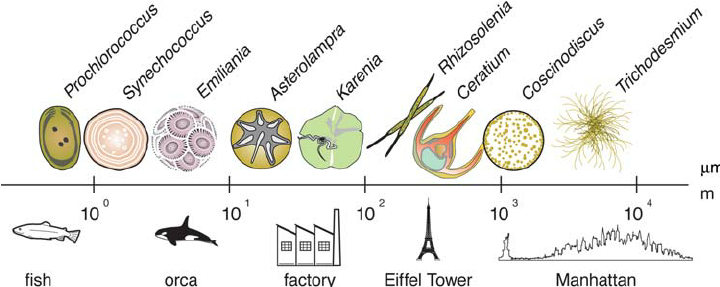
\includegraphics[trim = 0mm 0mm 0mm 0mm, clip, width=.9\linewidth]{./Chp1-Intro/SIZEphytoComparison_FinkelEtAl2010.png}
\caption[Scheme]{\small {"A comparison of the size range (maximum linear dimension) of phytoplankton
relative to macroscopic objects." from \cite{Finkel2010}}}
\label{FinkelPhySizeRange}
\end{figure}

The distribution of phytoplankton is driven by the complex physical forces that govern ocean currents and the chemistry of the bodies of water the move. The key components are macronutrients (e.g. nitrogen \& phosphorus) and micronutrients (e.g. iron \& cobalt) welling up from the deeper ocean or flushed in from continental sources. Wherever there are sufficient nutrients available within the euphotic zone, the depth where photosyntheticaly available radiation (PAR) is 1\% of the surface value, planktonic life begins to thrive. Ecosystems along continental margins provide a particularly productive habitat, with only 10\% of total ocean surface area covered by continental margins, but 10-15\% of marine primary production and more than 40\% of carbon export to the seabed occurring along coastal lines \citep{Yool2001,Muller-Karger2005}.


Phytoplankton growth indirectly feeds a considerable part of earth’s population through fisheries \citep{Stock2017} and even shapes the elemental composition of oceanic water itself \citep{Redfield1958}. 
The biomass produced is mostly consumed by higher trophic levels and either assimilated or excreted. Another large portion experiences natural mortality and viral lysis. Microbial degradation drives remineralization within the euphotic zone, which fuels regenerated production \citep{Eppley1979} [Perhaps put quotation about Microbial Loop here!]. 
A small fraction sinks out of the photic layer as fecal or detrital matter to the deeper ocean and an even smaller fraction reaches the sea floor as sediment ( 1 \%) and remains there over geological times \citep{Honjo2008}. This process has been termed the biological carbon pump. Carbon sequestered this way is removed from the ocean-atmosphere system for potentially millions of years. Given the projected rise of atmospheric CO$_2$ levels, it is of grave importance to understand how changes in the phytoplankton community at the surface, driven by anthropogenic stressors and climate change, will affect the carbon burial potential of oceanic ecosystems. 
Studies have both reported a global declining trend in marine primary production \citep{Boyce2012} and increasing trends in long-term ocean time series \citep{Chavez2011a}. 
In order to answer questions of how phytoplankton will respond to a changing climate it is necessary to look the diverse phytoplankton community in greater detail. 

\section{Characterizing phytoplankton}

Given the relevance of phytoplankton to the global 

How did Researchers start dealing with Phytoplankton?

Two approaches to isolate strains, or take bulk properties

Obviously bulk properties also have to be taken from specific depth

so this adds the problem of the complexity of the physical environment that is the ocean, with enormous volume, turbulunce mixing, diffusion and absorbance

I want to look at phytoplankton diversity, particularly from a functional type point of view. Quantify diversity as it relates to ecosystem function (as production for example).

The emergence of such a large range of organisms and the mechanisms sustaining their persistence has been one of the key topics in phytoplankton ecology over the last 50 years. Hutchinson's paradox.

"Moreover, major taxonomic groups of eukaryotic phyto- plankton can be classified into distinct functional groups (Iglesias-Rodriguez et al. 2002a) with unique biogeochemical signatures. Here, we combine the trait-based approach with the taxonomic sLASh phylogenetic information by broadly sam- pling relevant traits across major taxonomic groups of marine phytoplankton to gain new insights into the effects of evolutionary history on the physiological trait distribu- tions and community structure. An important aspect of a trait-based approach to
"community ecology is the trade-offs between traits (Tilman 1990; Grover 1991; Bohannan et al. 2002). When compe- tition for multiple resources is considered, species are thought to have trade-offs in their competitive ability for one vs. another nutrient (Tilman 1982) or for nutrient vs. light (Huisman \& Weissing 1994; Leibold 1997; Klausmeier \& Litchman 2001). Under non-equilibrium conditions, a trade-off between competitive ability and maximum growth rate may
Litchman, E., Klausmeier, C. A., Schofield, O. M., \& Falkowski, P. G. (2007). The role of functional traits and trade-offs in structuring phytoplankton communities: Scaling from cellular to ecosystem level. Ecology Letters, 10(12), 1170–1181. https:doi.org10.1111j.1461-0248.2007.01117.x


"Functional types can be composed of a large number of species with very different trait values, so the representation of a type by an average trait value may not be appropriate." (Irwin and Finkel 2018)
XXX

"Phytoplankton can be characterised by many morphological, physiological, behavioural and life history traits and trade-offs \citep{Litchman2008, Litchman2010}.

"Studies on the phytoplankton community composition and their response to the environmental gradients are not novel. Ramón Margalef was probably one of the first ecologist to give an important momentum to the topic.  \citep{Margalef1978} used observations of key traits, such as nutrient utilization and sinking rates, to support his well known concept called "Margalef's mandala". His classification of phytoplankton functional types (PFTs) at different nutrient and turbulent environmental conditions represents an excellent first example of how the trait-based notion can be applied to better understand phytoplankton community ecology, therefore setting up the stage for further developments in the field.


\subsection{Functional types and traits}

“Ecology has traditionally focused on species diversity as a way of characterizing the
health of an ecosystem. In recent years, however, the focus has increasingly shifted
towards trait diversity both within and across species” - from Functional Diversity Book

We have incredibly diverse Phytoplankton, and want to analyze traits and model -> need to simplify somehow => Functional Types

so I want to talk about:
that phytoplankton can be divided in functional groups
talk about the Work that Finkel and Irwin have done! 
question whether it makes sense to use functional types instead of species, …
Thus, photopigment-based measures offer an efficient way to quantify community or functional diversity (X Moreno et al., 2012 X). (From Pinckney et al 2015)



XXXX


XXXX


XXXX


\section{Modeling phytoplankton communities}
Going into the details is necessary to understand the whole picture

One tool of integration are mathematical models

Given the complexity of the ocean ecosystem, it is necessary to aggregate our knowledge of the many smaller parts into comprehensive ecological models in order to understand the full-scale implications. 

Computational models of phytoplankton growth have been developed since the 1970s and have greatly increased in sophistication and complexity since then, co-evolving with the rise in computational resources. Ecosystem modelling started with simple box-model descriptions of a few trophic levels. These were the nutrient-phytoplankton-zooplankton (NPZ) and nutrient-phytoplankton-zooplankton-detritus (NPZD) models, which succeeded in reproducing the basic bloom dynamics observed in the temperate ocean (Evans 1988, Fasham et al. 1990). However, in their generalistic approach, these models unavoidably limit the characterization of a diverse phytoplankton community (Bruggeman 2009). To make up for this shortcoming, in the following two decades, these models were expanded to more complex plankton functional type (PFT) models (Le Quere et al. 2005). 

For every group of species that fulfill a distinct ecosystem function, a new set of parameters was added, complicating the model structure and massively prolonging calculations. This somewhat intuitive approach of having every functional group represented in a model, however, did create problems. First and foremost, this is the lack and inherent uncertainty of data from field and culture experiments to constrain functional types. 

This again leads to the difficulty of validating the model output in light of insufficient information (Shimoda et al. 2016 ).Trait-based modeling, on the other side, tries to circumvent the problem of biodiversity (i.e. complexity) in natural systems with a radically different approach. The interactions of phytoplankton with their environment are based on multiple traits which characterize generalized physiological properties like nutrient affinities or motility. Ideally, these traits can be directly measured and are independent of species and therefore they can be directly related to the properties of the organisms function within the ecosystem, such as nutrient affinity for example deally, these traits can be directly measured and are independent of species and therefore they can be directly related to the properties of the organisms function within the ecosystem, such as nutrient affinity for example (Litchman and Klausmeier 2008).  


A simple example of a trait-based description of phytoplankton succession is scaling the maximal nutrient acquisition rate and the respective affinity with cell size. A trade-off would emerge between different size classes, allowing for a modeled succession along gradients of nutrient depletion. One example of a very similar approach is the PhytoSFDM model developed by Acevedo-Trejos and colleagues (Acevedo‐Trejos et al. 2013, Acevedo-Trejos et al. 2015). In their approach, the trait-based modelling of phytoplankton is even further simplified, by describing an entire community as a size- distribution with a mean value and a variance, instead of modeling all the different size classes explicitly. This moment-based structure further simplifies the mathematical basis of the model, and leads to much faster processing times and less uncertainty in parameter estimation.



"quite a few publications using models go too far in their extrapolations, whilst the general discussion still strongly revolves around meaningful model structures.. but no consensus is anywhere to be seen!
"need to identify the basic uncertainties and see if there is a way to discuss them scientifically
"Michaelis Menten kinetics are really outdated.. and i suppose using them in a trait-based modelling approach is questionable just the same
"plankton ecosystems are typically highly aggregated, a single variable gives the response of an incredibly diverse assemblage of phytoplankton species (P. Franks, 2009)


\begin{figure}
\centering
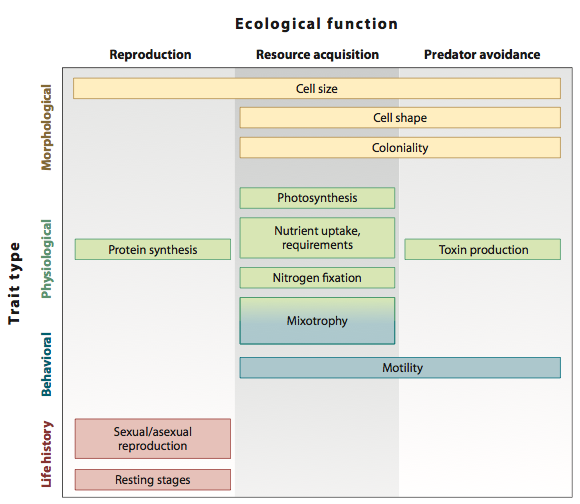
\includegraphics[width=0.7\linewidth]{./Chp1-Intro/Fig_litchman2008.png}
\caption[Scheme]{\small{Phytoplankton functional traits. Taken from \citet{Litchman2008}}}
\label{phytotrait}
\end{figure}

XXX

XXX

XXX

XXX. 

XXX

XXX

ALWAYS NEED A GOOD BASIS IN DATA TO VALIDATE MODELS AND HYPOTHESES

\section{The Cariaco basin \& the CARIACO time series}

A coastal tropical ecosystem

"continental margins constitute only about 10\% of the total ocean surface area, these regions are responsible for about 10–15\% of the global marine primary production and greater than 40\% of seabed carbon sequestration (Yool and Fasham, 2001; Muller-Karger et al., 2005). 
"The Cariaco Basin, located off the coast of Venezuela, has been the site of high frequency water column sampling for marine biogeochemical and ecological observations since 1995. The observations were collected as part of the Cariaco Ocean Time-Series Program (Muller-Karger et al., 2001; Thunell et al., 2007). 

XXXX

In addition to the recent importance of the cariaco basin as the site of an important paleo-oceanographic time sereis, the Cariaco basin has served as a natureal laboratory for biogeochemists for over 50 years. This basin has been key in constructiong stoichiometric models of organic matter remineralization (Redfield et al 1963 and Richards 1975!), developing residence time and box models, and numerous other studies.

\begin{figure}
\centering
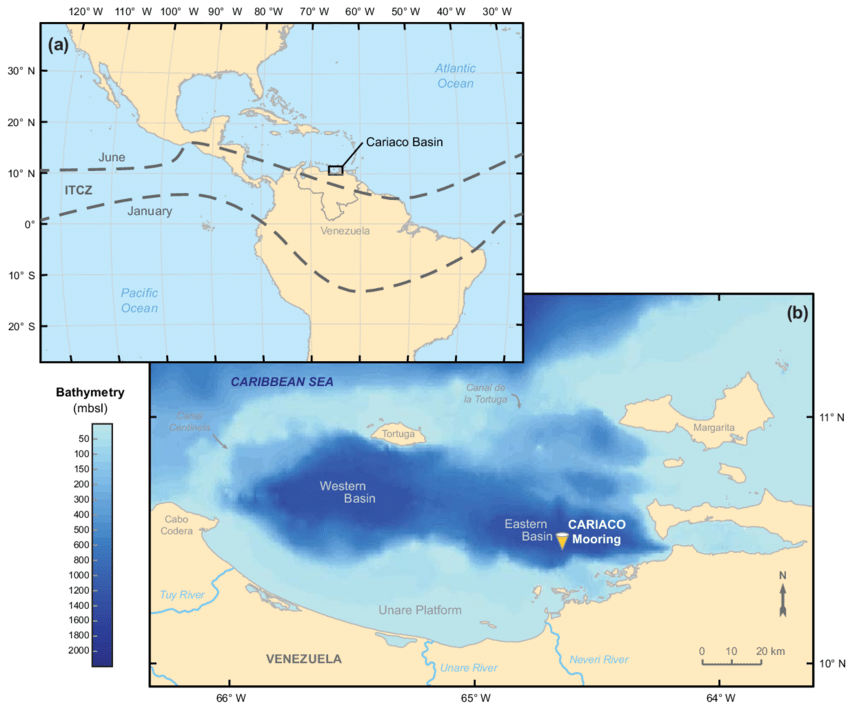
\includegraphics[trim = 0mm 0mm 0mm 0mm, clip, width=1.\linewidth]{./Chp1-Intro/CARIACObasinMAP_Bringueetal2018.png}
\caption[Scheme]{\small {"Study area. A. Location of the Cariaco Basin off the Venezuelan coast in the southern Caribbean Sea, with January and June positions of the Intertropical Convergence Zone (ITCZ). B. Location of the CARIACO station in the eastern sub-basin, general bathymetry and local rivers emptying in the basin (bathymetric data from GEBCO\_08 Grid)" from \cite{Bringue2019}}}
\label{CARIACO-map}
\end{figure}

XXXX

XXX

THEN TALK ABOUT THE COLLABorDATASHARE WITH JPINCKNEY AND CBENITEZNELSON, and how this allows an even deeper look at the biomass dynamics


\section{Aims of the proposed PhD project}
"The general goal of my Ph.D. project is to study the processes that structure the phytoplankton community in contrasting environmental regions of the Atlantic Ocean, using a trait-based modelling perspective. The specific aims during the course of the project are to:

\begin{itemize}
\item MANUSCRIPT 1 "Understanding Shifts in CARIACO"
\item MANUSCRIPT 2 "technical paper" - Geoscientific Model development
\item MANUSCRIPT 3 "BDEF in CARIACO"
\end{itemize}


\chapter{A trait-based characterization of phytoplankton communities in contrasting environmental regions of the Atlantic Ocean}

\small {\textbf{Manuscript to be submitted to Marine Ecology Progress Series}}

%\subsection*{}
%\textbf{ABSTRACT}: In recent years trait-based ecology studies had been providing new insights on the mechanisms driving natural variation based on measurable key characteristics of organisms. Here we investigate the phytoplankton community size-composition in the Atlantic Ocean using data from the Atlantic Meridional Transect program. We extended the existing knowledge on the distribution of the phytoplankton size composition in the Atlantic, using a larger data set, integrating phytoplankton size composition, nutrients concentrations, and grazers abundance into a trait-based approach. The selected subset was constrain by k-means partitioning and based on the prevailing environmental conditions. Also we studied how the different phytoplankton size fractions respond to different environmental gradients. Our results suggest a linkage of the \textit{in situ} environmental conditions with community size-composition, and regardless of the spatio-temporal conditions. We discuss how the observed patterns of phytoplankton size-fractions in the Atlantic Ocean are coherent with the niche partitioning theory and opposed to the unified neutral theory of biodiversity.

\normalsize
\section{Introduction}
For decades ecologists have been trying to understand how the structure of phytoplankton communities is associated to the environmental conditions, with a particular focus on the causes and consequences of natural variation. One of the approaches adopted in this important quest is based on observations of key characteristics of organisms, populations or communities. These key characteristics are also called traits \citep{McGill2006, Violle2007}. Trait-based ecology aims at developing an understanding and a better predictability of natural communities by linking traits that influence organism performance and fitness to prevailing environmental conditions \citep{McGill2006}. 

Phytoplankton communities are ideal systems for the application of a trait-based approach. They are relatively simple and have well defined ecological niches, which are determined by physical and environmental conditions, by resource allocation strategies, and by inter-specific relationships \citep{Litchman2007}. Phytoplankton organisms have various well-understood morphological, physiological, behavioural, and life history traits. Among a number of potentially relevant traits, cell size is probably the one that can best characterize phytoplankton communities, because many ecophysiological processes such as nutrient and light acquisition and resistance to grazing are significantly correlated with cell size \citep{Litchman2008,Litchman2010}. A variety of these traits are frequently measured \textit{in vivo} and \textit{in situ} due to the global importance of phytoplankton as a primary producer with a significant influence on the marine food-webs and on the biogeochemical cycles of major nutrients\citep{Falkowski1998}.

Since 1995 two scientific cruises of the Atlantic Meridional Transect (AMT) Programme have crossed the Atlantic Ocean from Plymouth (UK) to South America or South Africa almost every spring and autumn. The information collected during these cruises includes data on size-fractionated chlorophyll-a, on the concentrations of nitrate, nitrite, phosphate and silicate, on temperature, and on zooplankton abundances. The spatial extent of the transects, that cross a range of ecosystems from sub-polar to tropical and from euphotic shelf seas and upwelling systems to oligotrophic mid-ocean gyres, and the richness of the variables observed, make the dataset important for studying the size compositions of phytoplankton communities and the processes shaping them at an ocean basin scale. Previous analyses have focused on a description of the occurrences of the different size fractions \citep{Maranon2001}, but did not consider the direct influence of environmental conditions on the community structure. A more comprehensive analysis that includes the most recent observations and integrates the relevant environmental data with the available phytoplankton community size fractions is to our knowledge still lacking. The work we present here therefore intends to investigate the mechanisms determining the phytoplankton community structure in regions of contrasting environmental conditions (i.e. regions with different nutrient, temperature, and grazing regimes).

We broaden previous analyses by considering a larger and most up-to-date selection of data than any previous study. More specifically, we integrate phytoplankton size-fractions with temperature, various nutrient concentrations, and zooplankton abundances in a first attempt to disentangle the relative contribution of bottom-up and top-down processes in shaping the size structure of the phytoplankton community.

The first step in our analysis is to spatially separate the selected AMT dataset according to the well-established ecological classification of the world ocean by \citet{Longhurst2006}. In a second step, we classify the phytoplankton communities by using only the corresponding nutrients and temperature data and compare the results with the classification of \citet{Longhurst2006}. In a last step, we relate the environmental differences to the cell size compositions in order to highlight the emergent patterns of community structures at the ocean basin scale.

\section{Methods}

\begin{figure}
\centering
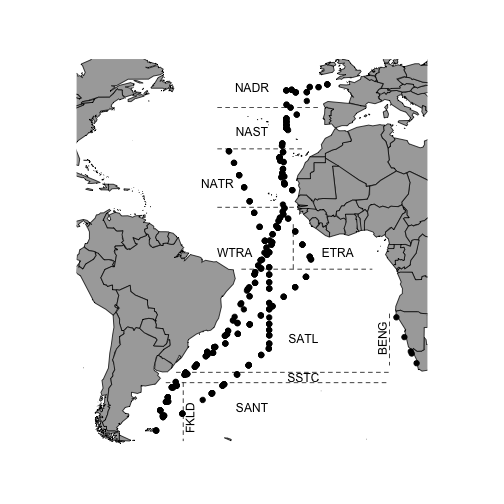
\includegraphics[trim = 30mm 20mm 25mm 20mm, clip, width=0.5\linewidth]{./Chp2-Pre/amt_mapFINAL2.png}
\caption[Scheme]{\small {The AMT subset of 410 samples used in this study. The dashed lines represent the simplified limits of the Longhurst (2006) ecological provinces.}}
\label{Map}
\end{figure}

We collected a number of observed variables from the AMT Programme (www.amt-uk.org). The resulting dataset comprised size fractionated chlorophyll-a (phytoplankton size fractions hereafter), nitrate+nitrite, phosphate and silicate concentrations, temperature, and zooplankton abundance (considered as a qualitative indication of grazing pressure). We restricted our selection to the mixed layer depth, defined as the depth at which a variation of 0.5 $^\circ$C in temperature and of 0.125 in density is observed with respect to the surface value (i.e. the value at 5-10 m depth). The resulting dataset included 410 samples from a total of 9 AMT cruises (from AMT2 to AMT6, AMT10, AMT11, AMT13, and AMT14). These cruises took place in April-May or September-October of 1996 (AMT2 and AMT3), 1997 (AMT4 and AMT5), 1998 (AMT6), 2000 (AMT10 -AMT11), and 2003 (AMT13 and AMT14). 

During most of the cruises the phytoplankton size fractions were in the range of 0.2-2 $\mu$m (picoplankton), 2 -20 $\mu$m (nanoplankton), and $>$20 $\mu$m (microplankon), although AMT13 and AMT14 measured four size classes (0.2-2, 2-5 5-10, $>$10 $\mu$m). For consistency, we considered the 2-5 and 5-10 $\mu$m size classes as part of the nanoplankton and the $>$10 $\mu$m class as part of the microplankton. The three size fractions were then normalized according to the proportion of each size fraction to the total chlorophyll-a concentration.

The selected dataset covered temperate, subtropical and tropical regions of the Atlantic Ocean (Figure \ref{Map}). Following Longhurst's (\citeyear{Longhurst2006}) classification, ten ecological provinces were sampled by the AMT cruises: four temperate provinces, comprising of the North Atlantic Drift (NADR; 24 samples), the South Subtropical Convergence (SSTC, n=21), the Subantartic Water Ring (SANT, n=14), and the Falkland Island (FKLD; 52 samples); two subtropical provinces, comprising of the North Atlantic Subtropical Gyral (NAST; 37 samples) and the South Atlantic Subtropical Gyral (SATL, 129 samples); three tropical provinces, the North Atlantic Tropical Gyral (NATR, 51 samples), the Eastern Tropical Atlantic (ETRA, 13 samples) and the Western Tropical Atlantic (WTRA, 64 samples); and one upwelling region, the Benguela province (BENG, 5 samples). With this dataset the phytoplankton community size composition was analyzed by means of a linear mixed effect model (LME) to test if the community size-structure differs among ecological provinces. The ecological provinces were classified into regions, defined as: temperate (NADR, FKLD, SSTC, SANT), tropical (NATR, WTRA, ETRA), subtropical (SATL, NAST) and upwelling (BENG). The model was fitted to the data using the size fractions and the regions as fixed factors, and the ecological provinces as randomly varying factors.

We utilized a cluster analysis based on the $k$-means algorithm (a statistical method that partitions $n$ observations into $k$ clusters in which each observation belongs to the cluster with the nearest mean) to alternatively classify the data with respect to the prevailing environmental conditions. The environmental variables considered were nitrate+nitrite, phosphate and silicate concentrations, and temperature. 

We also applied a principal component analysis (PCA) to the environmental variables and the normalized size fractions to assess the effect of a specific environmental gradient to changes in the phytoplankton size fractions. We quantified the linear relationships between the environmental data and the size-structure information. 

In addition, we quantified the relation of the three size fractions to the grazer abundance relatively to AMT3 and AMT5, because zooplankton data were only available for these two cruises. These analyses were carried out using R v2.12.2 (The R Foundation for Statistical Computing, 2011).

\section{Results}

\begin{figure}
\centering
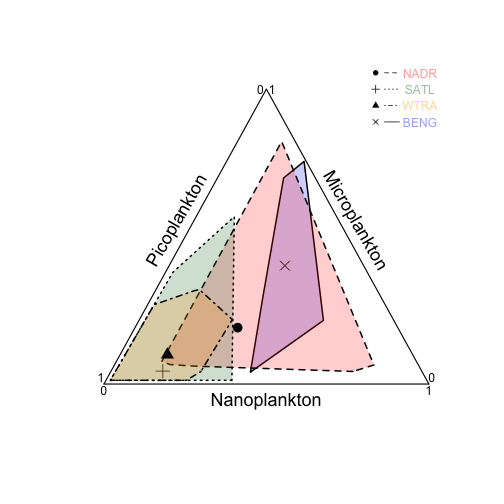
\includegraphics[trim = 20mm 30mm 20mm 20mm, clip, width=0.6\linewidth]{./Chp2-Pre/amt_4RegionsTriSizeFrac4.png}
\caption[Scheme]{\small {Phytoplankton community size structure of four ecological provinces in the Atlantic Ocean. The contours correspond to the convex hull of the size-fraction distribution of each province. The symbols indicate the corresponding mean values.}}
\label{RegSizeFrac}
\end{figure}

\begin{figure}
\centering
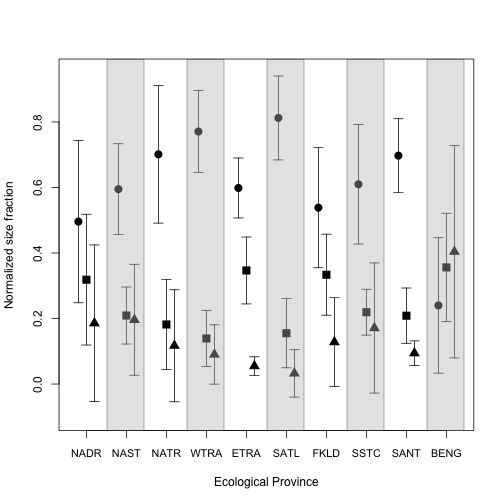
\includegraphics[trim = 0mm 0mm 0mm 0mm, clip, width=0.9\linewidth]{./Chp2-Pre/amt_MeanSDProvinces.png}
\caption[Scheme]{\small {Relative mean abundances ($\pm$sd) of three phytoplankton size fractions of ten ecological provinces of the Atlantic Ocean. The symbols indicate the mean values of the normalized size fractions: picoplankton (\ding{108}), nanoplankton(\ding{110}) and microplankton (\ding{115}).}}
\label{means}
\end{figure}

The size-structure of the phytoplankton communities is highly variable in different ecological provinces of the Atlantic Ocean (Figure \ref{RegSizeFrac}). When the mean size-fraction of only four selected provinces are compared, an increasing trend towards bigger phytoplankton sizes can be observed from the warmer provinces of the tropics and subtropics to the colder provinces of, for example, the Benguela upwelling. In tropical and subtropical waters (such as WTRA and SATL), picoplankton is the most common size class, with only a few occurrences of nano- and microplankton. In contrast, temperate provinces such as NADR are characterised by a more heterogeneous distribution of size classes and the upwelling province is dominated mainly by pico- and microplankton. Provinces located in the temperate regions have a larger cell size variability, as indicated by the larger standard deviation there than in the provinces located in the tropical regions (Figure \ref{means}). These differences are rather significant for the picoplankton (LME/anova, df=3, F=6.6315, p=0.0247) and the microplankton (LME/anova, df=3, F=5.5189,p=0.0368) size fractions, while they are less significant for the nanoplankton (LME/anova, df=3, F=2.03341, p=0.2108) size fractions.

\begin{figure}
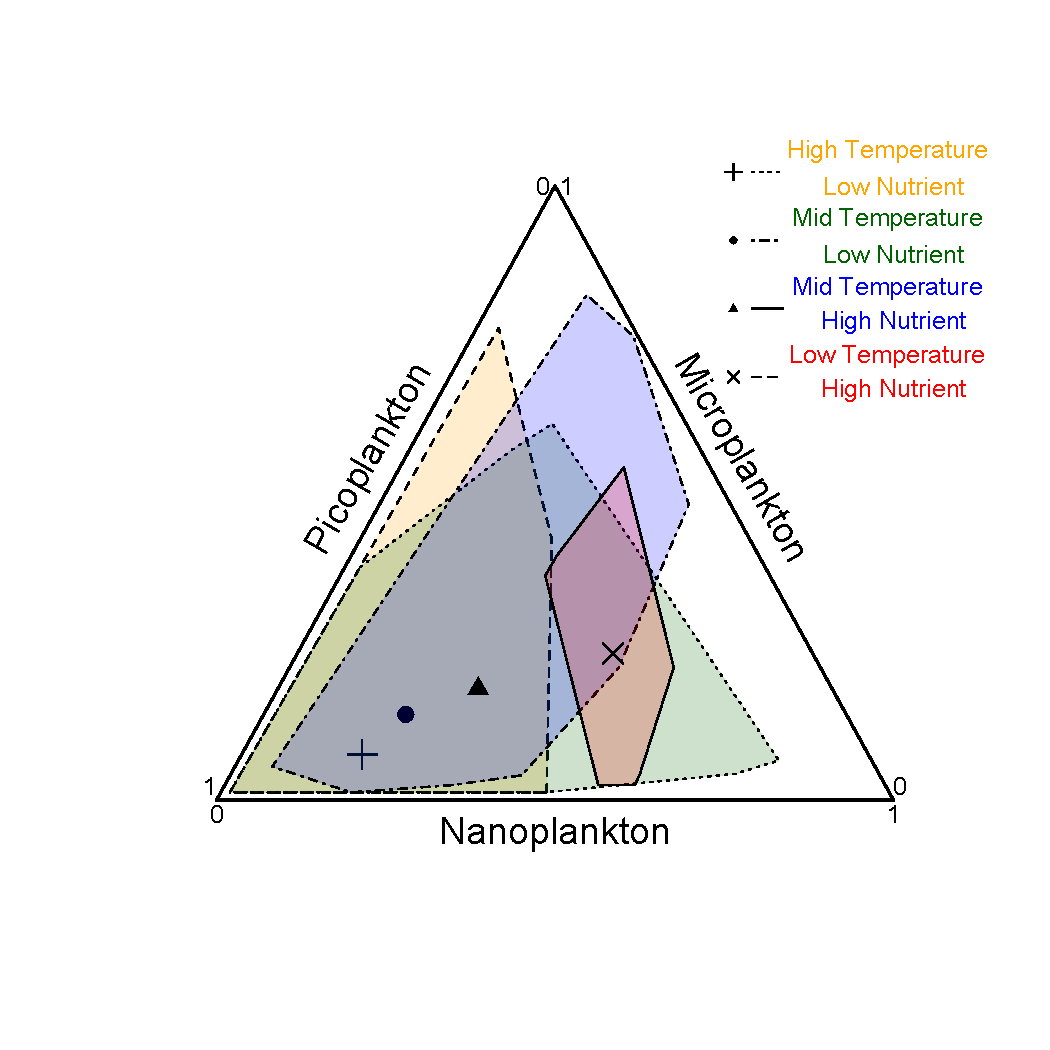
\includegraphics[trim = 12mm 15mm 10mm 15mm, clip, width=0.5\linewidth]{./Chp2-Pre/amt_clsEnvFINAL4-5.pdf}
\put(1,210){\textbf{b)}}
\put(-180,210){\textbf{a)}}
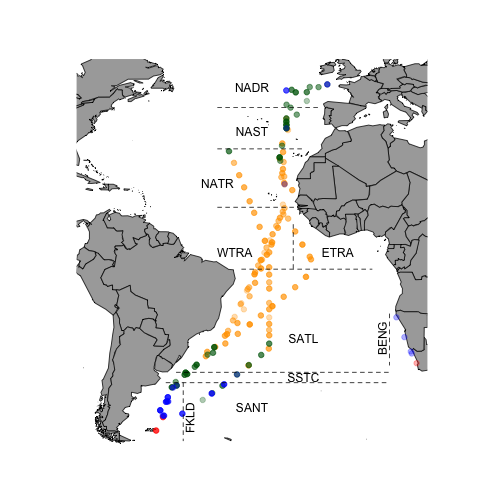
\includegraphics[trim = 20mm 20mm 20mm 20mm, clip, width=0.5\linewidth]{./Chp2-Pre/amt_mapClsEnv3.png}
\caption[Scheme]{\small {Phytoplankton community size structure and environmental conditions. a) Distributions of size-classes clustered according to water temperature and nutrient concentration with contours corresponding to the convex hull of the size-fraction distribution of each cluster; symbols denoting the mean values of the size fractions. b) Geographical distribution of the clusters compared to Longhurst provinces. The colour coding reflects the cluster classification.}}
\label{clusters}
\end{figure}

\begin{table}
\centering
\caption[Scheme]{\small {Mean values of environmental parameters for the different clusters: High temperature - Low nutrients (HTLN), Mid temperature - Low nutrients (MTLN), Mid temperature - High nutrients (MTHN and Low temperature - High nutrients (LTHN).}}
\label{tableclus}
\begin{tabular} {c c c c c}
cluster & NO$_2^-$ + NO$_3^-$ & PO$_4^{3-}$ & SiO$_4^{2-}$ & Temperature \\ \hline
HTLN & 0.150$\pm$0.575 & 0.064$\pm$0.078 & 1.097$\pm$0.575 & 25.299$\pm$2.000 \\
MTLN & 0.556$\pm$1.102 & 0.112$\pm$0.141 & 0.816$\pm$0.617 & 17.894$\pm$2.191 \\
MTHN & 9.027$\pm$3.593 & 0.799$\pm$0.373 & 2.423$\pm$1.375 & 11.925$\pm$2.797 \\
LTHN & 30.324$\pm$4.549 & 1.336$\pm$0.208 & 4.590$\pm$1.926 & 6.810$\pm$3.435 \\ \hline
\end{tabular}
\end{table}

The $k$-means clustering analyses of temperature, nitrate+nitrite, phosphate, and silicate concentrations reveals that regions between 30$^{\circ}$ North and South share similar environmental characteristics of high temperatures and low nutrient concentrations (HTLN, yellow dots in Figure \ref{clusters}b, cf. Table \ref{tableclus}). Observations from temperate provinces are clearly separated from HTLN data. They are categorized into three clusters: Mid temperature - Low nutrients, Mid temperature - High nutrients and Low temperature - High nutrients (respectively green, blue and red dots in Figure \ref{clusters}b, cf. Table \ref{tableclus} ). In summary, we obtained a new classification of the data into four regions, which explains 87.3\% of the variance. The mean size of phytoplankton in the four clusters indicates an increasing trend from the high-temperature, low-nutrient region towards the low-temperature, high-nutrient regions (Figure \ref{clusters}a). The PCA on all data shows highest loadings for temperature (positive loading) and nitrate+nitrite concentration (negative loading) with respect to the first principal component (Figure \ref{PrinComp}). Furthermore, the relative occurrence of picoplankton is positively correlated with temperature, while nutrient concentrations are positively correlated with occurrences of nano- and microplankton (Figure \ref{PrinComp}).

The results of the regression analyses of all data show that phytoplankton size composition varies with the environmental conditions irrespective of temporal changes (see Figure \ref{response1} and Table \ref{stats}). A shift from a picoplankton dominated community towards a nano- and microplankton dominated community occurs with increasing nutrient concentrations (see Figure \ref{response1}a, \ref{response1}b and \ref{response1}c). By contrast, the relative abundance of picoplankton increases from about 40\% to about 80\% with a temperature increase from 4.8-9$^{\circ}$C to 25-29$^{\circ}$C, whereas the fractions of nano- and microplankton decreases by about 50\%.

When restricting the regression analysis to the only two cruises that also sampled zooplankton (AMT3 and AMT5), we observe an increase in copepod abundance in association to a decline in the relative occurrence of picoplankton from 70$\%$ to less than 40$\%$ and an increase of the relative occurrence of nanoplankton from 20$\%$ to 60$\%$. The microplankton size fraction is, however, not affected by changes in the zooplankton abundance (Figure \ref{response2}).

\begin{figure}
\centering
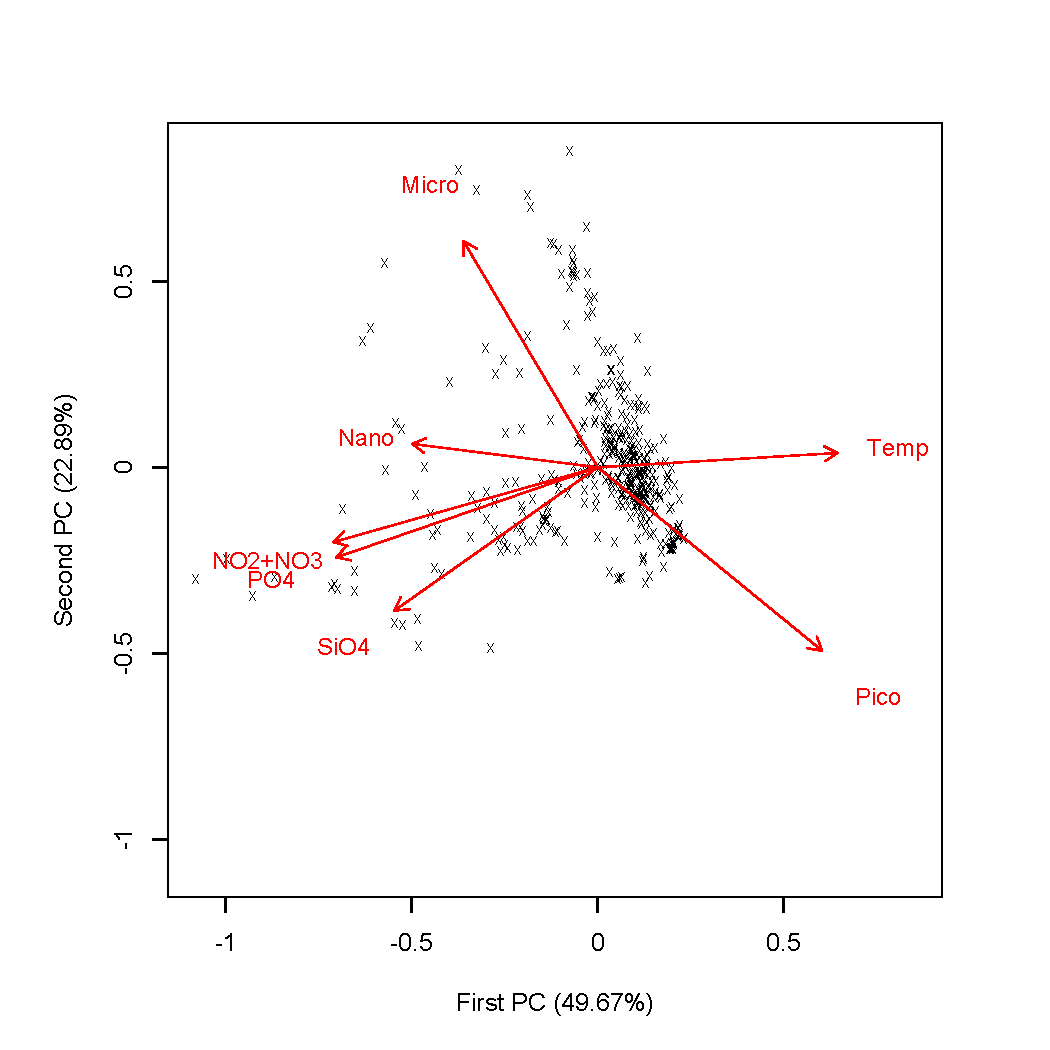
\includegraphics[trim = 0mm 0mm 0mm 0mm, clip, width=0.9\linewidth]{./Chp2-Pre/amt_PrinComp.pdf}
\caption[Scheme]{\small {Principal Component Analysis of environmental parameters and normalized phytoplankton size fractions.}}
\label{PrinComp}
\end{figure}

\begin{figure}
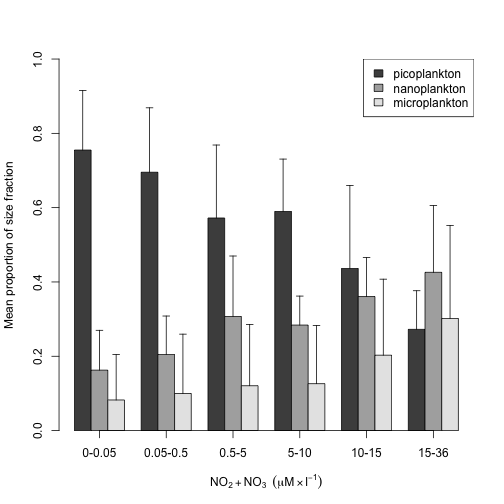
\includegraphics[trim = 0mm 0mm 0mm 15mm, clip, width=0.5\linewidth]{./Chp2-Pre/amt_NO3_bars2.png}
\put(-180,210){\textbf{a)}}
\put(1,210){\textbf{b)}}
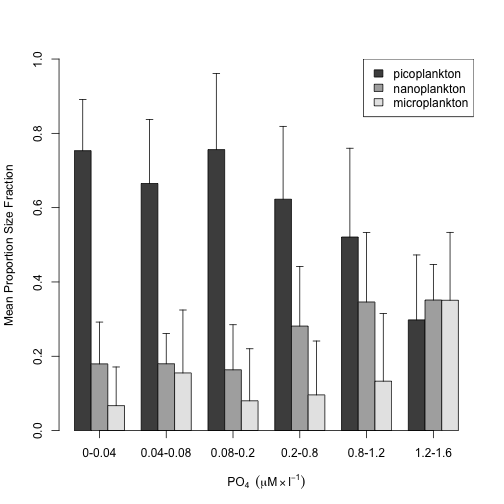
\includegraphics[trim = 0mm 0mm 0mm 15mm, clip, width=0.5\linewidth]{./Chp2-Pre/amt_PO4_bars2.png}
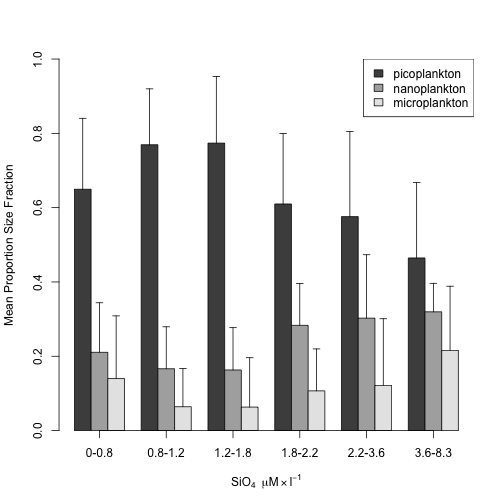
\includegraphics[trim = 0mm 0mm 0mm 15mm, clip, width=0.5\linewidth]{./Chp2-Pre/amt_SiO4_bars2.png}
\put(-180,210){\textbf{c)}}
\put(1,210){\textbf{d)}}
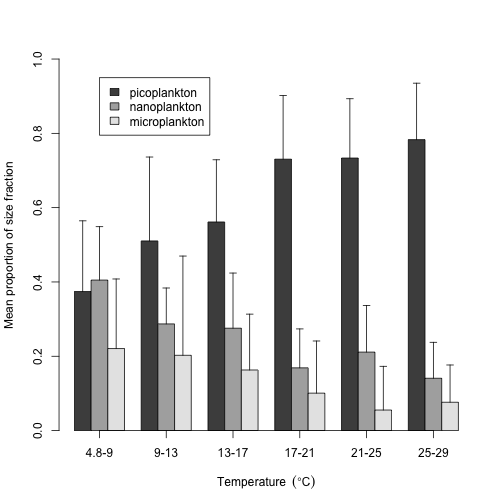
\includegraphics[trim = 0mm 0mm 0mm 15mm, clip, width=0.5\linewidth]{./Chp2-Pre/amt_Temp_bars2.png}
\caption[Scheme]{\small {Relative composition of picoplankton, nanoplankton and microplankton size fractions changing with concentrations of nitrate+nitrite (a), phosphate (b), and silicate (c) and with temperature (d). The bars represent mean values and the error bars indicate the standard deviation.}}
\label{response1}
\end{figure}

\begin{figure}
\centering
\includegraphics[trim = 0mm 0mm 0mm 15mm, clip, width=0.6\linewidth]{./Chp2-Pre/amt_zoo_bars2.png}
\caption[Scheme]{\small {Relative composition of picoplankton, nanoplankton and microplankton size fractions changing with copepod abundance. The bars represent mean values and the error bars indicate the standard deviation.}}
\label{response2}
\end{figure}

\begin{table}
\centering
\caption[Scheme]{\small {Summary statistics for linear fittings of the three size fractions to each environmental variable.}}
\label{stats}
\begin{tabular} {c c c c c c c c c c }
& \multicolumn{3} {c} {Picoplankton} & \multicolumn{3} {c} {Nanoplankton} & \multicolumn{3} {c} {Microplankton} \\
& slope & p-value & $r^2$ & slope & p-value & $r^2$ & slope & p-value & $r^2$ \\ \hline
NO$_2^-$ + NO$_3^-$ &-0.090 &0.002 & 0.908 &0.050 &0.001 & 0.921 &0.040 &0.010 &0.792 \\
PO$_4^{3-}$ &-0.0812 &0.021 &0.711 &0.042 &0.012 &0.777 &0.039 &0.125 &0.354 \\
SiO$_4^{2-}$ &-0.047 &0.085 &0.455 &0.030 &0.044 &0.597 &0.016 &0.247 &0.142 \\ 
Temperature &0.082 &0.001 &0.914 &-0.047 &0.008 &0.812 &-0.035 &0.003 &0.885 \\
Copepods &-0.063 &0.064 &0.520 &0.068 &0.051 &0.567 &-0.004 &0.788 &-0.222\\ \hline
\end{tabular}
\end{table}


\section{Discussion}
We analyzed cruise data from different regions of the Atlantic Ocean covering mainly two seasons (late spring/early summer and autumn) in the period 1996 to 2003. Our results showed, consistently with the geographical classification of \citet{Longhurst2006} (Figures \ref{RegSizeFrac} and \ref{means}), patterns of phytoplankton size distributions characterized by the dominance of picoplankton in oligotrophic (SATL) and tropical (e.g. WTRA) waters and by the dominance of larger size classes in nutrient-rich waters (BENG). These patterns are also consistent with the works of \citet{Maranon2000, Maranon2001, Poulton2006, Moreno-Ostos2011, Huete-Ortega2011}. Our new classification method, based on the prevailing environmental conditions (Figure \ref{clusters}) and independent from spatial and temporal information, maximizes differences of the environmental properties among clusters of data and generates patterns of phytoplankton size distributions similar to the ones obtained by the Longhurst's classification, which uses a richer and spatially informed dataset. The value of our approach is therefore in the fact that it leads to results consistent with the present day understanding of phytoplankton biogeography and ecology of the Atlantic without requiring information on the geographical and temporal origin of the data. Our finding also proves the generality and robustness of the trait-based approach and confirms the sensitivity of phytoplankton cell size to environmental conditions and possibly (because of the paucity of zooplankton data) to grazing pressure. In fact, the phytoplankton size compositions resulted to be strongly associated with prevailing environmental conditions (Figures \ref{response1} and \ref{response2}). Furthermore, the consistency of our results with similar previous studies of the Atlantic Ocean that used either less AMT data than our study \citep{Maranon2000, Maranon2001, Poulton2006} or data from sources different than the AMT cruises \citep{Moreno-Ostos2011, Huete-Ortega2011} suggests that the different phytoplankton size structures observed are robust features of the Atlantic Ocean.

The results we obtained with the clustering technique (Figure \ref{clusters}) revealed that the areas between 30$^\circ$ N and 30$^\circ$ S are characterized by nutrient and temperature regimes that give picoplankton a competitive advantage over larger phytoplankton. In contrast, a wider range of phytoplankton size classes distinguishes colder waters with high nutrient concentrations.

Smaller phytoplankton cell sizes have a competitive advantage over larger phytoplankton under low nutrient, low light and low grazing pressure \citep{Litchman2008, Litchman2010}. From our regression analyses (Figures \ref{response1} and \ref{response2}) we inferred a strong control of NO$_3^-$+NO$_2^-$ and temperature on all three size fractions. Pico- and nanoplankton size fractions, however, appeared more sensitive to changes in PO$_4^{3-}$, SiO$_4^{2-}$ and copepod abundance. We propose that these effects are caused by a trade-off between resource acquisition and predation pressure, although with the caveat represented by the paucity of the zooplankton data and by the qualitative value we attribute to zooplankton abundance as an indication of grazing pressure. There are a number of important physiological and ecological processes that strongly depend on phytoplankton cell size \citep{Kiorboe1993, Cermeno2008a, Finkel2009a}, including metabolic rates, maximum nutrient uptake rate, nutrient diffusion, light absorption, sinking velocity, trophic interactions and even diversity within taxa, which is often a log-normal distribution of body size. Our results are therefore consistent with this general "size rule" \citep{Finkel2009a}. To our knowledge it is the first time that this feature is observed in data extending across an entire ocean basin and irrespective of temporal changes.

Our size-based analyses therefore substantiate remarkable properties of the variation of a key trait at an ocean basin scale. Moreover, these findings are corroborating Baas Becking's tenet "everything is everywhere, but the environment selects" \citep{BaasBecking1934} over a large-scale environmental gradient. Here we evidenced how the partitioning of resources along our selected trait, phytoplankton size, is a strong feature at an ocean basin scale. These observations lend weight to arguments supporting the niche partitioning theory rather than the unified neutral theory of biodiversity. The importance of the finding that the prevailing environmental condition is the major driver of the phytoplankton community structure in the Atlantic Ocean need to be further investigated using the trait-based modelling approach of \citet{Bruggeman2007, Merico2009}. This modelling tool will help to disentangle the relative contributions of the top-down vs. bottom-up processes in shaping the phytoplankton community structure, a research direction also promoted very recently by \citet{Follows2011}.

\section{Acknowledgements}
This study uses data from the Atlantic Meridional Transect Consortium (NER/0\\/5/2001/00680), provided by the British Oceanographic Data Centre and supported by the Natural Environment Research Council. 


\chapter{PhytoMFTM - a flexible object-oriented PFT model}


\small {\textbf{This is the work towards the second manuscript, to be submitted to Geoscientific Model Development (GMD)}}


\normalsize
\section{Python ecosystem model package development}
General intro sentence" 

Tao of open science for ecology: \citep{Hampton2015}
the concept of transparency at all stages of the scientific process

Important role of bioinformatics in ecology, as an ever evolving discipling: \citep{Michener2012}

A number of general-purpose simulation toolkits are in use today, in the form of specialized programming languages (Fritzson and Engelson, URL), software libraries (Fishwick, 1995, Minar et al., 1996, Lorek and Sonneschein, 1998) or pre-packaged models that a flexible parameter choice makes suitable to represent a large number of situations within a particular field (e.g. Klenner et al., 1997). Also, various simulation interoperability ‘blackboards’ have been developed over the last few years. Examples are FRAMES (PNNL, URL), DIAS (ANL, URL), HLA (DMSO, URL), MMS (Leavesley and Restepo, 1995). While many of these solutions have been successful in a restricted field, the lack of a strong and general declarative framework (along with platform dependency and often awkward installation and use) has made them unsuitable for easy and general adoption by a wide modelling community. In comparison, a few highly successful and widely used simulation tools (Stella: HPS, 1995, Costanza et al., 1998; Powersim: Powersim Co., URL) have privileged the ease of use of well-developed graphical interfaces, at the cost of restricting their application to the limits imposed by the interface itself and the adoption of a single modelling paradigm. In most modern science, application of such tools is usually limited to prototyping, as they are unsuitable for large-scale simulation and model integration.
\citep{Villa2001} <- this is the quote above
 
why would this be interesting to anyone else


movement towards open source programming languages

As funding agencies embrace open science principles that encourage sharing data and computer code developed to produce research outputs, we must respond with new modes of publication.

Open Source, Open Access, Open Science!
comparability

!!!!cite a nice pushing for this publication here!!!!

Necessity of standardisation of methods and open publishing of data and models: \citep{Reichman2011}
Focus on sharing data openly, but just as important is publishing of statistical scripts and actual model code!

This only makes sense if model code is understandable to the average ecosystem modeler, need to use a widely available, standardized programming language:
PYTHON
programming language of the future for earth sciences \citep{Lin2012}

also well documented open source packages can play an important role in teaching computational literacy to university students \citep{Farrell2018}



teach PhD Students from the ground up to code their own models in Python, as of yet there is a lack of coherent ressources. Definitely cite the PhytoMFTM model and publication \citep{AcevedoTrejos2016}

extensible framework
bb



XXX

\section{Methods}



\subsection{Object-oriented structure}
Explain Code structure, with some nice graphicx
XXX

XXXX

\subsection{Model formulation and usage}
xXXX

explain how to run the model!

XXXX

XXXX

XXX


End Methods here


\chapter {Further work}

\section{Size-based model}

\subsection{Background}

Phytoplankton organisms are significantly limited by nutrient diffusion and by sinking. These two crucial processes in water pose important constraints on phytoplankton morphological traits such as cell size. Cell size is therefore subject to an important selection pressure that tends to favour those shapes and sizes that allow phytoplankton access nutrient resources more efficiently while maintaining themselves in the surface waters to access light \citep{Litchman2008}. Size plays also a major role in growth and metabolism \citep{Finkel2009a}. The importance of this trait has motivated the development of a number of size-based ecological models. For example, \citet{Baird2007} developed a 1D, size-based model of three major group of organisms (phytoplankton, protozoan and metazoan) that takes into account a certain number of size-classes. Each of these classes of organisms could be further subdivided into defined functional groups or species that can be mathematically represented with state variables. Baird and Suthers' (\citeyear{Baird2007}) model is formulated independently of the number of size classes, this help to reduce the complexity in terms of number of state variables and free parameters. However, with increasing number of size classes the model becomes computationally more expensive without any apparent benefit in the understanding of the system dynamics and with a clear increase in model sensitivity. Although size-based, which is still an unusual practice in phytoplankton modelling, this approach follows the typical tendency of introducing extra complexity in models, beyond the simple nutrient-phytoplankton-zooplankton-detritus (NPZD) configurations, when more size classes are considered. This tendency, however, faces numerous difficulties, particularly because of the poorly understood ecology, the lack of data, the problems connected with aggregating diversity within functional groups into meaningful state variables and constants, and the higher sensitivity of outputs to the parameterizations in question \citep{Anderson2005}.

Interesting alternatives to this modelling practice are obtained if principles of the Dynamic Energy Budget theory (DEB) of \citet{Kooijman2009} and trait-based approaches are considered into plankton models. DEB theory attempts to build a quantitative background in one of the most fundamental processes in biology, the individual metabolism. The key principles on which this theory is based are: the conservation of mass and energy, the general applicability to all possible species (its not species-specific), the structure of metabolic modules (reservoirs and structures), the consistency with empirical data, the simple model specification (Occam's razor) and the capacity of organisms to increase the control of their metabolism (strong, weak, structural acquisition and thermal homeostasis) \citep{Sousa2010}.  

\begin{figure}
\centering
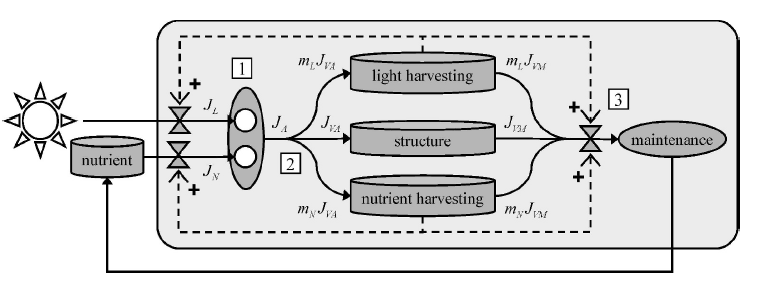
\includegraphics[trim = 0mm 0mm 0mm 0mm, clip, width=1\linewidth]{./Chp3-Further/Bruggeman-2007.png}
\caption[Scheme]{\small {Bruggeman and Kooijman model scheme. Taken from \citet{Bruggeman2007}}}
\label{Bruggeman}
\end{figure}

In 2007 \citet{Bruggeman2007} developed a trait model based on DEB concepts to study phytoplankton diversity and succession. The model (\ref{Bruggeman}) captures the seasonal dynamics of the phytoplankton community structure and key process which influence diversity, such as migration. However, they had to face the problem of having to consider too many species (and therefore too many state variables and parameters) when tackling biodiversity studies. \citet{Bruggeman2007}, however, elegantly resolved the problem by approximating the full model with a simpler one. Using a moment closure technique to estimate the few, most important macroscopic properties of the full, complex system, such as total biomass, mean trait value, and trait variance, as previously proposed by \citet{Wirtz1996, Norberg2001}, Bruggeman and Kooijman's(\citeyear{Bruggeman2007}) obtained a simpler model, which dynamics compared remarkably well with the one of the full model. It should be noted, however, that this method assumes a normal distribution of the trait possibly omitting interesting multimodal dynamics \citep{Bruggeman2007}. Following studies refined this approach by providing a complete mechanistic framework for developing these kind of models and by confirming the quality of the approximation in capturing the essential physiological and ecological characteristics of the full model \citep{Merico2009}. 

\subsection{Method}
The main focus of my PhD work is to develop a size-based model following the approaches of  \citet{Bruggeman2007, Merico2009} in order to further explore the detailed mechanisms leading to the observed phytoplankton size structure distributions in regions of the Atlantic Ocean of contrasting environmental conditions. The guiding principle for defining the traits and the tradeoffs to be incorporated into my model will be based on the concept that organisms face trade-offs in their ability to allocate limited energy and resources to growth, reproduction and defence, which is central to most theories explaining the diversity of life on Earth \citep{Tilman2000}. Based on available observations, I will therefore develop a trade-off between competitive ability for nutrient acquisition and resistance to grazing (\ref{model}). I will then include a specific grazing pressure that relates to both phyto- and zooplankton mortalities.

The resulting, full size-based model will be approximated with a simpler model of aggregate macroscopic properties using the moment closure approximation proposed by \citet{Wirtz1996, Norberg2001} and further refined by \citet{Bruggeman2007, Merico2009}. The phytoplankton total biomass ($P$), the mean trait ($\bar{s}$), and the trait variance ($v$) will be formulated as follows:

\begin{align*}
\frac{dP}{dt} & = \left[r(\bar{s})+\frac{1}{2}v\frac{\partial^{2} r(\bar{s})}{\partial s^{2}}\right]P \nonumber \\
& \nonumber \\
\frac{d\bar{s}}{dt} & = v\frac{\partial r(\bar{s})}{\partial s}\nonumber \\
&\nonumber \\
\frac{dv}{dt} & = v^{2}\frac{\partial^{2} r(\bar{s})}{\partial s^{2}}\nonumber\\
\end{align*}

The approach of defining a trade-off that relates size to the competitive ability for nutrient acquisition and resistance to predation \citep{Merico2009} leads to mechanistically capture bottom-up (nutrient availability and acquisition capabilities) versus top-down (avoid grazing) processes, major shaping forces of a phytoplankton community. The model will be tested against and constrained by the AMT observations on environmental data and community size structures in the Atlantic Ocean (chapter 2).  

\begin{figure}
\centering
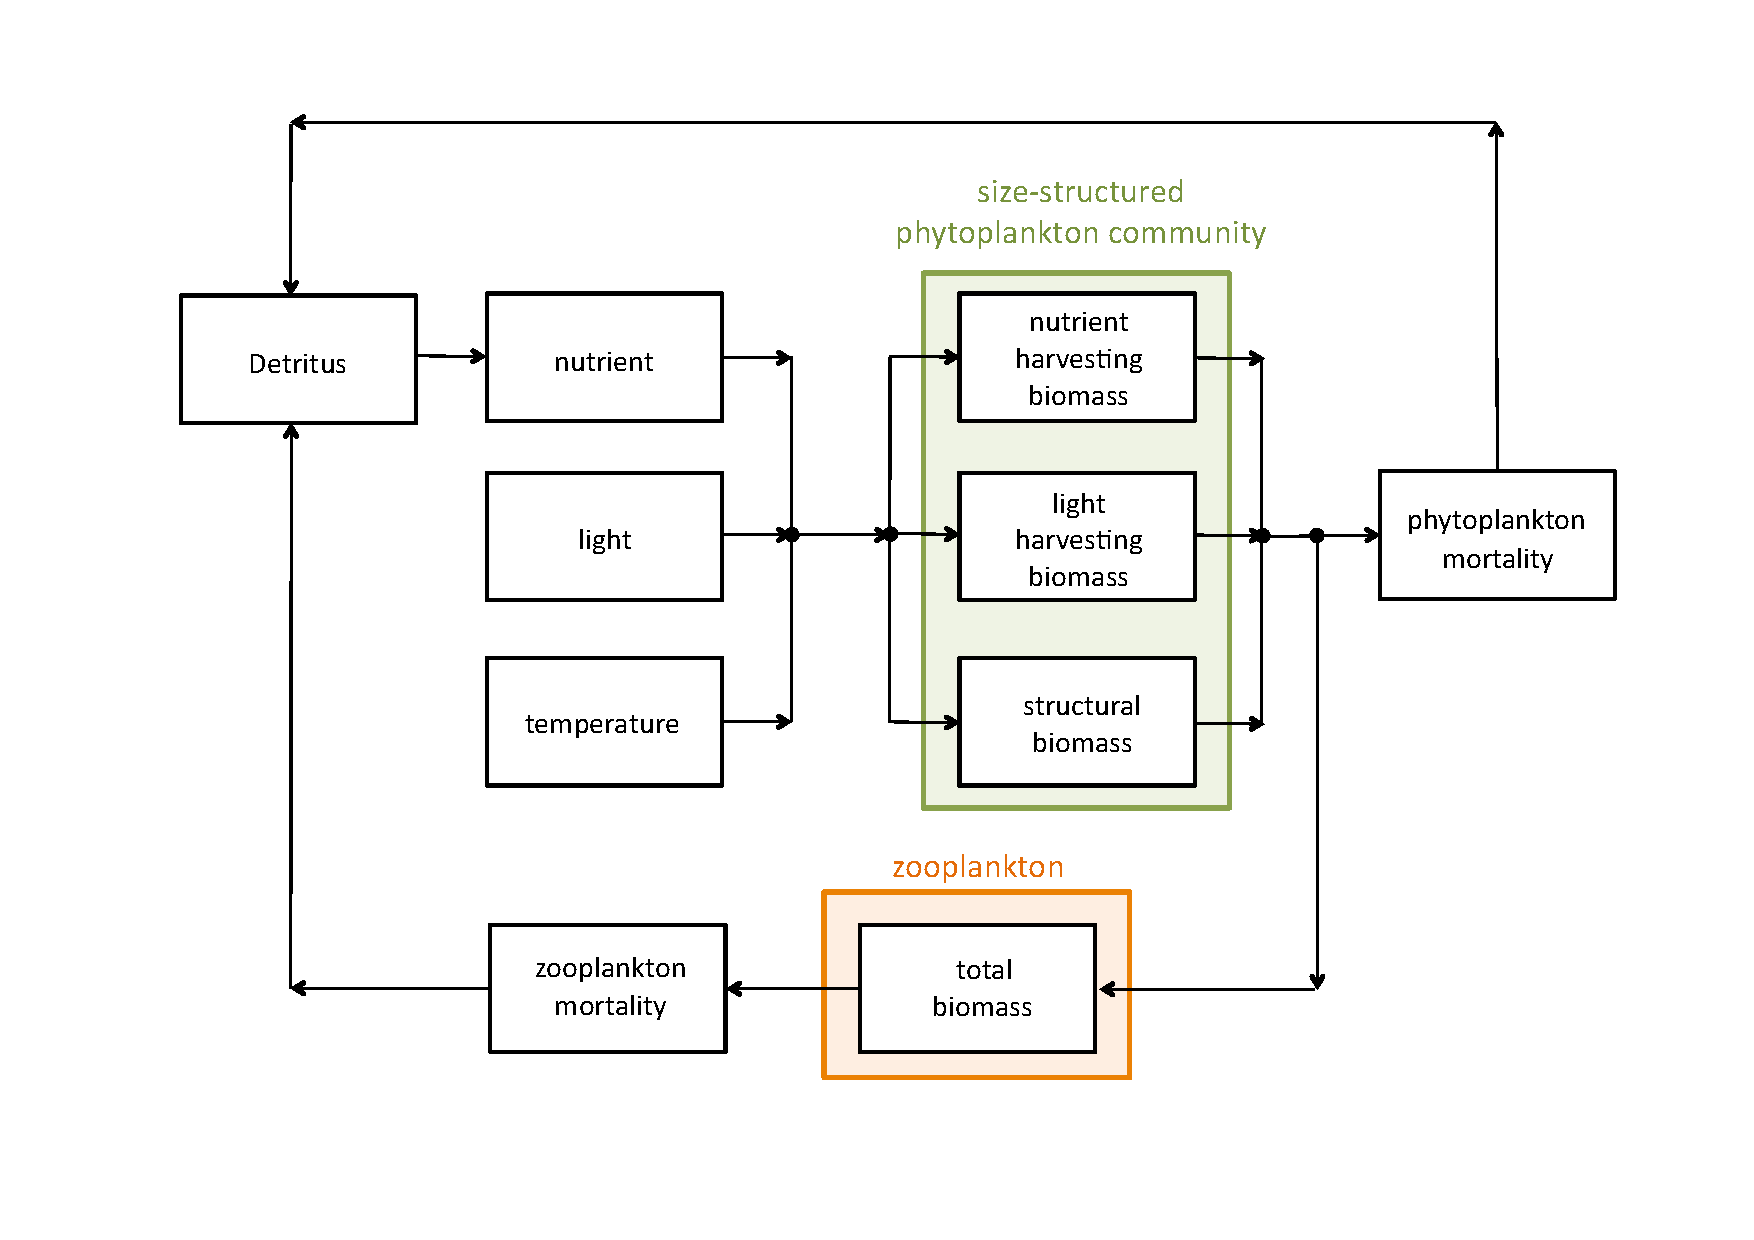
\includegraphics[trim = 15mm 50mm 15mm 25mm, clip, width=1\linewidth]{./Chp3-Further/model-scheme.pdf}
\caption[Scheme]{\small {Scheme of the proposed size-based model. In this model phytoplankton allocates energy (or biomass) to different pools such as nutrient and light harvesting biomasses and generic structural biomass. A certain fraction of the phytoplankton biomass flows into the zooplankton biomass and a remaining fraction is remineralized into the nutrient pool}}
\label{model}
\end{figure}

\subsection{Relevance}
The work proposed with this PhD project will be important for further developing trait-based models of planktonic communities. Previous studies have not been able to consistently address complex adaptive systems with a reduced amount of complexity. The ability to model a complex system as a single adaptive entity while retaining the most fundamental ecological processes shaping its dynamics is doubtlessly elegant and attractive. 

As shown in chapter 2, different regions in the Atlantic Ocean have specific community patterns. With my model I will attempt to capture the observed community structures regions of the Atlantic Ocean with contrasting environmental conditions. To our knowledge no effort have been made yet to develop such a trait-based model in this region of the world. As typical of any modelling study, my work will provide also quantitative understanding of the relative contribution of the most important physiological and ecological processes shaping the phytoplankton community size structure. 

A key aspect with our approach is that under any given environmental condition, typical community size-structures will emerge consistently to the Bass Becking's principle that "Everything is everywhere, but the environment selects" \citep{BaasBecking1934}. More generally, I expect that this work will provide the possibility to test different ecological hypothesis proposed for explaining biodiversity, including the niche and the neutral hypotheses \citep{Hubbell2001,Mcgill2003}.

\section{Multi-trait size-based model}
A recent review on the current developments of plankton models by \citet{Follows2011} stress that most of the trait-based models elaborated so far have been only focusing on photoautotroph. It appears reasonable to start extend trait-based formulations also to other groups such as zooplankton, as in our proposed size-based model (\ref{model}). I will therefore extend my model to include a dynamic selection of the prey based on the size of predator.

I believe that the allometric scaling of predator-prey interactions in planktonic systems is a key aspect for further advances in trait-based models due to the importance of this process in regulating the phytoplankton community structure\citep{Agrawal2001, Litchman2008}. Technically, I will mechanistically derive two trade-off functions, one for the phytoplankton as explained in the previous section, and the other for the zooplankton. The new trade-off function will be based on the size of the zooplankton and on the size of the predated phytoplankton. The type of model approximation used will be the once estimated from the moment closure, in analogy to the size-based model proposed in section 3.1.2.

With this multi-trait implementation we expect to reduce the parameterization and overall complexity of early models possibly leading to a significant advance in plankton ecosystems modeling by developing a more parsimonious mechanistic description.

\section{Paleo-reconstruction of planktonic communities}

\begin{figure}
\centering
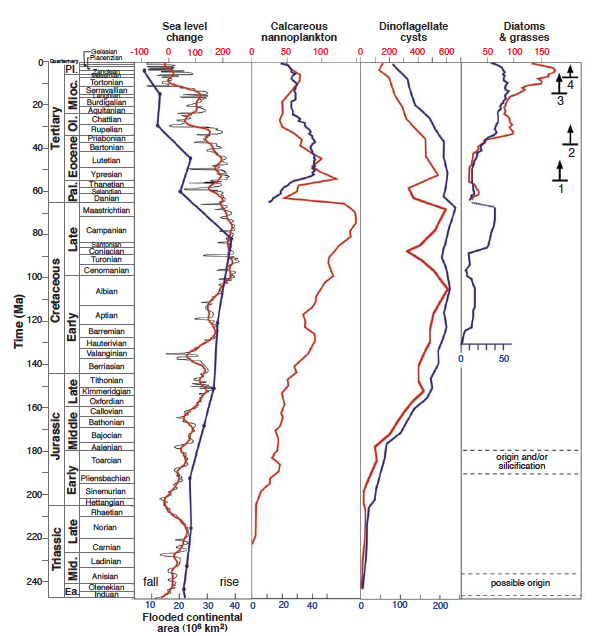
\includegraphics[trim = 0mm 0mm 0mm 0mm, clip, width=1\linewidth]{./Chp3-Further/Falkowski-2004.png}
\caption[Scheme]{\small {Comparison of major phytoplankton groups with sea-level change. The red line accounts for species diversities from published studies. The blue line accounts for the genus diversity compiled from public databases by the authors. Taken from \citet{Falkowski2004a}. }}
\label{Falkowski}
\end{figure}

Since Darwin times, ecologist have tried to understand the evolutionary processes that lead to the current patterns of biodiversity. \citet{Hutchinson1961} was fascinated by the capacity of phytoplankton communities to produce such  a large diversity from a limited range of resources fro which they compete. In the history of life on Earth, phytoplankton emerged at around 2.5 billion years ago when cyanobacteria started to spread in the earth oceans, thus creating an enormous impact on the global environment. Later $\sim$ 1.6-1.8 billion years ago, unicelular eukaryotes raised when they started to "use" prokaryotic cells as their metabolic slaves. From that point on, different kind of unicellular eukaryotes emerged, until three characteristic groups of phytoplankters originated from an ancestral red alga, and started to dominate earths aquatic environments (Figure \ref{Falkowski}) \citep{Falkowski2004a}. Since the Middle Triassic these well know groups, dinoflagellates, coccolithophores and diatoms, began to play an important role on the biogeochemistry of our planet and supported a wide range of life forms in more and more complex food webs \citep{Falkowski1998}.

\citet{Jiang2005,Litchman2009} develop a size-based evolutionary model, based on game theory, to determine the driving processes which could produce  the difference size distributions of diatoms. Their model results suggest the nitrogen to phosporus stoichiometric ratio, the nutrient fluctuation, and the changes on mixed layer depth, as major mechanisms leading the size differences in diatoms. 

Following these approaches, I plan to adopt my trait-based modelling approach to study the changes in the phytoplankton community composition during the Cenozoic period. This approach will be based on the size-based model developed for the Atlantic Ocean but obviously appropriately set up for targeting environmental changes operating on a geological time scale. The species diversity will be mechanistically captured in my model  by the variance of the trait distribution, and the prevaling mean trait value at a specific time will give an indication of the characteristic group or species dominating the community. Due to the distinct morphological differences in the three functional groups, it is appropriate to use size as a key trait to disentangle the different mechanisms shaping phytoplankton diversity across the Cenozoic era. 

\newpage

\section{Time table} 

\begin{figure}[h]
\centering
\includegraphics[trim = 20mm 25mm 20mm 25mm, clip, width=1\linewidth]{./Chp3-Further/Chronogram.pdf}
\end{figure}



\bibliographystyle{meps.bst} 
\begin{footnotesize}
\bibliography{proposal.bib}
\end{footnotesize}

%REMOVE THIS LATER%
%%% FIGURES %%%

\begin{figure}
\centering
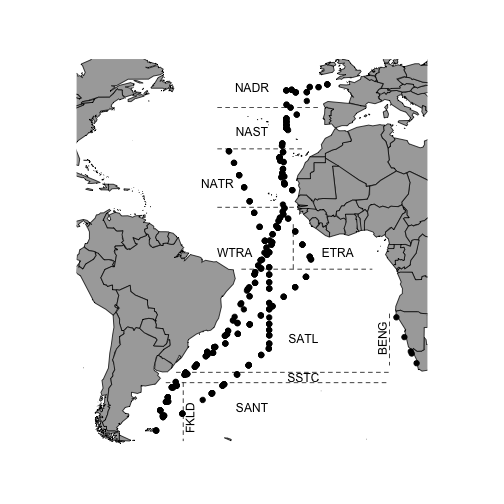
\includegraphics[trim = 30mm 20mm 25mm 20mm, clip, width=0.5\linewidth]{./Chp2-Pre/amt_mapFINAL2.png}
\caption[Scheme]{\small {The AMT subset of 410 samples used in this study. The dashed lines represent the simplified limits of the Longhurst (2006) ecological provinces.}}
\label{Map}
\end{figure}

\begin{figure}
\centering
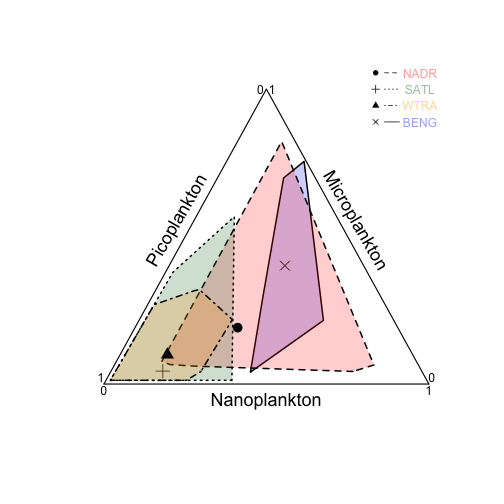
\includegraphics[trim = 20mm 30mm 20mm 20mm, clip, width=0.6\linewidth]{./Chp2-Pre/amt_4RegionsTriSizeFrac4.png}
\caption[Scheme]{\small {Phytoplankton community size structure of four ecological provinces in the Atlantic Ocean. The contours correspond to the convex hull of the size-fraction distribution of each province. The symbols indicate the corresponding mean values.}}
\label{RegSizeFrac}
\end{figure}

\begin{figure}
\centering
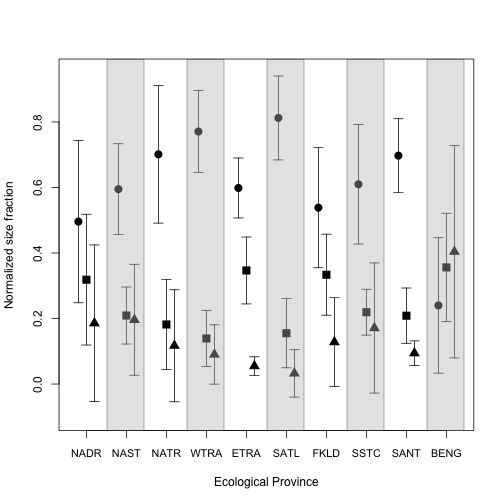
\includegraphics[trim = 0mm 0mm 0mm 0mm, clip, width=0.9\linewidth]{./Chp2-Pre/amt_MeanSDProvinces.png}
\caption[Scheme]{\small {Relative mean abundances ($\pm$sd) of three phytoplankton size fractions of ten ecological provinces of the Atlantic Ocean. The symbols indicate the mean values of the normalized size fractions: picoplankton (\ding{108}), nanoplankton(\ding{110}) and microplankton (\ding{115}).}}
\label{means}
\end{figure}

\begin{figure}
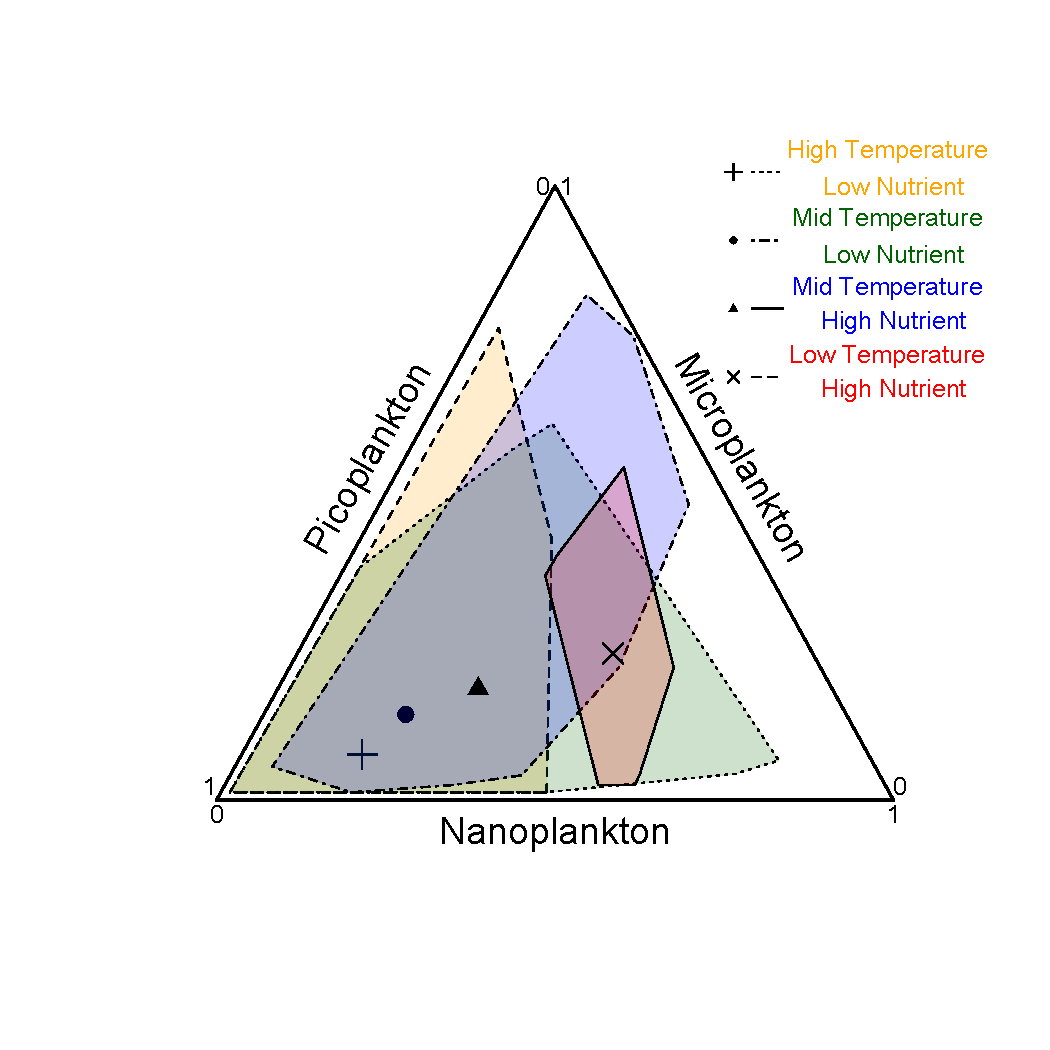
\includegraphics[trim = 12mm 15mm 10mm 15mm, clip, width=0.5\linewidth]{./Chp2-Pre/amt_clsEnvFINAL4-5.pdf}
\put(1,210){\textbf{b)}}
\put(-180,210){\textbf{a)}}
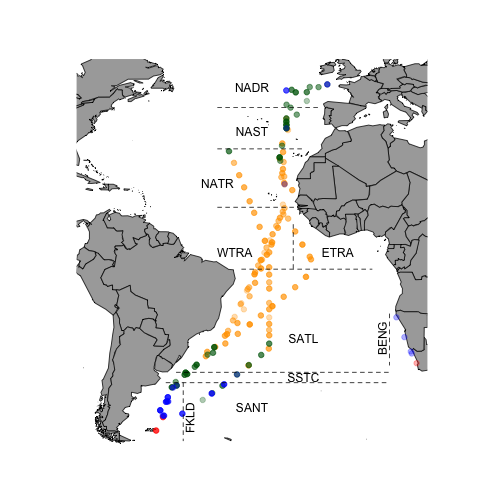
\includegraphics[trim = 20mm 20mm 20mm 20mm, clip, width=0.5\linewidth]{./Chp2-Pre/amt_mapClsEnv3.png}
\caption[Scheme]{\small {Caption comes here my friend""""""".}}
\label{clusters}
\end{figure}


\begin{figure}
\centering
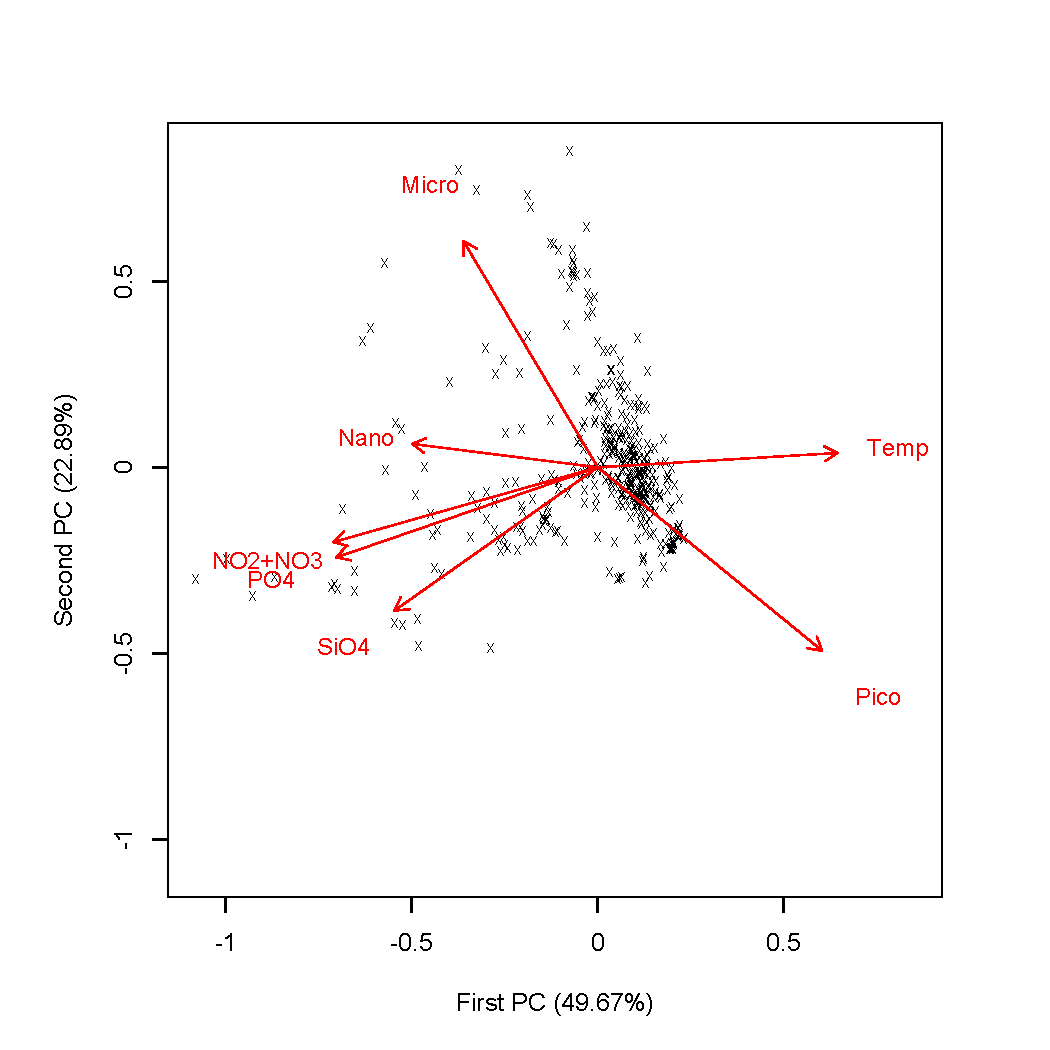
\includegraphics[trim = 0mm 0mm 0mm 0mm, clip, width=0.9\linewidth]{./Chp2-Pre/amt_PrinComp.pdf}
\caption[Scheme]{\small {Principal Component Analysis of environmental parameters and normalized phytoplankton size fractions.}}
\label{PrinComp}
\end{figure}

\begin{figure}
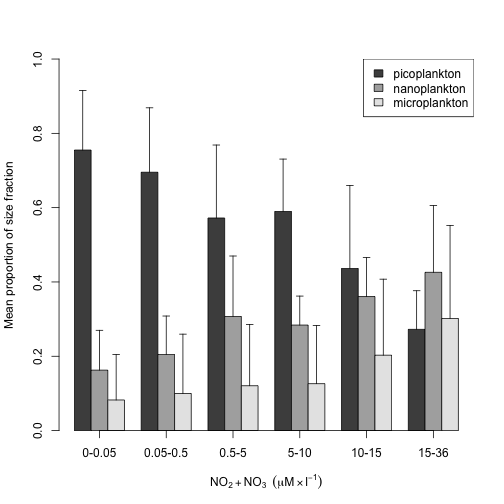
\includegraphics[trim = 0mm 0mm 0mm 15mm, clip, width=0.5\linewidth]{./Chp2-Pre/amt_NO3_bars2.png}
\put(-180,210){\textbf{a)}}
\put(1,210){\textbf{b)}}
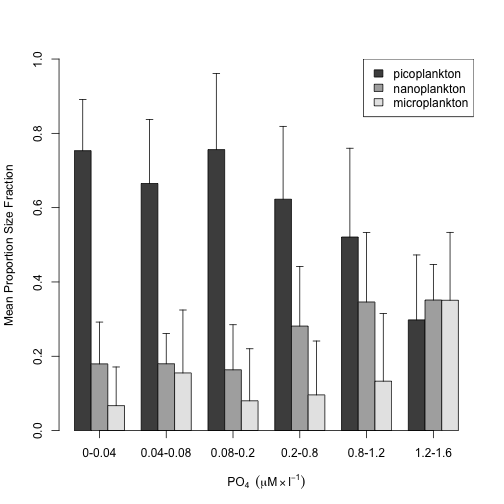
\includegraphics[trim = 0mm 0mm 0mm 15mm, clip, width=0.5\linewidth]{./Chp2-Pre/amt_PO4_bars2.png}
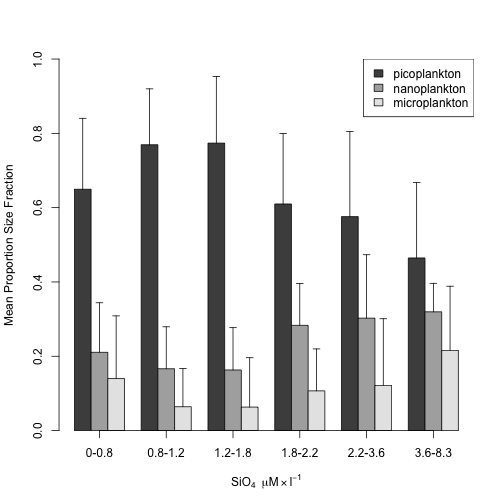
\includegraphics[trim = 0mm 0mm 0mm 15mm, clip, width=0.5\linewidth]{./Chp2-Pre/amt_SiO4_bars2.png}
\put(-180,210){\textbf{c)}}
\put(1,210){\textbf{d)}}
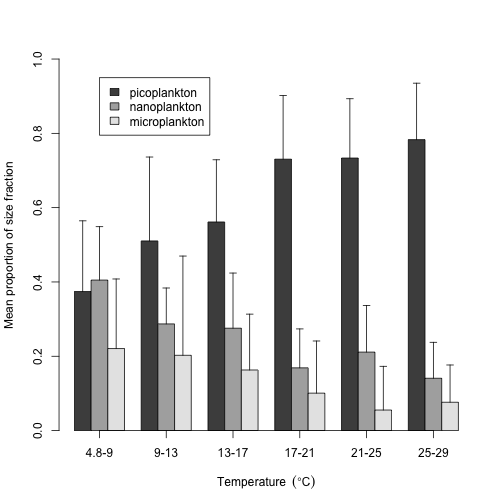
\includegraphics[trim = 0mm 0mm 0mm 15mm, clip, width=0.5\linewidth]{./Chp2-Pre/amt_Temp_bars2.png}
\caption[Scheme]{\small {Relative composition of picoplankton, nanoplankton and microplankton size fractions changing with concentrations of nitrate+nitrite (a), phosphate (b), and silicate (c) and with temperature (d). The bars represent mean values and the error bars indicate the standard deviation.}}
\label{response1}
\end{figure}

\begin{figure}
\centering
\includegraphics[trim = 0mm 0mm 0mm 15mm, clip, width=0.6\linewidth]{./Chp2-Pre/amt_zoo_bars2.png}
\caption[Scheme]{\small {Relative composition of picoplankton, nanoplankton and microplankton size fractions changing with copepod abundance. The bars represent mean values and the error bars indicate the standard deviation.}}
\label{response2}
\end{figure}

\begin{figure}
\centering
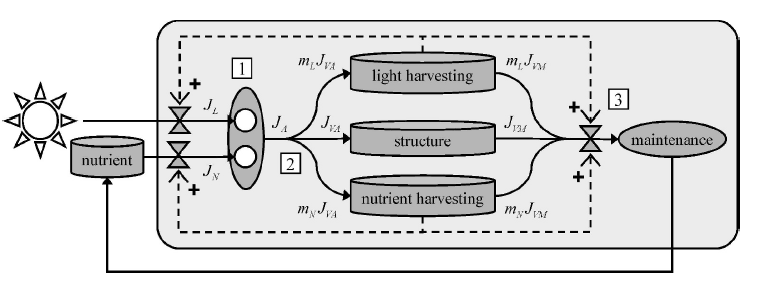
\includegraphics[trim = 0mm 0mm 0mm 0mm, clip, width=1\linewidth]{./Chp3-Further/Bruggeman-2007.png}
\caption[Scheme]{\small {Bruggeman and Kooijman model scheme. Taken from \citet{Bruggeman2007}}}
\label{Bruggeman}
\end{figure}


\begin{align*}
\frac{dP}{dt} & = \left[r(\bar{s})+\frac{1}{2}v\frac{\partial^{2} r(\bar{s})}{\partial s^{2}}\right]P \nonumber \\
& \nonumber \\
\frac{d\bar{s}}{dt} & = v\frac{\partial r(\bar{s})}{\partial s}\nonumber \\
&\nonumber \\
\frac{dv}{dt} & = v^{2}\frac{\partial^{2} r(\bar{s})}{\partial s^{2}}\nonumber\\
\end{align*}

The approach of defining a trade-off that relates size to the competitive ability for nutrient acquisition and resistance to predation \citep{Merico2009} leads to mechanistically capture bottom-up (nutrient availability and acquisition capabilities) versus top-down (avoid grazing) processes, major shaping forces of a phytoplankton community. The model will be tested against and constrained by the AMT observations on environmental data and community size structures in the Atlantic Ocean (chapter 2).  

\begin{figure}
\centering
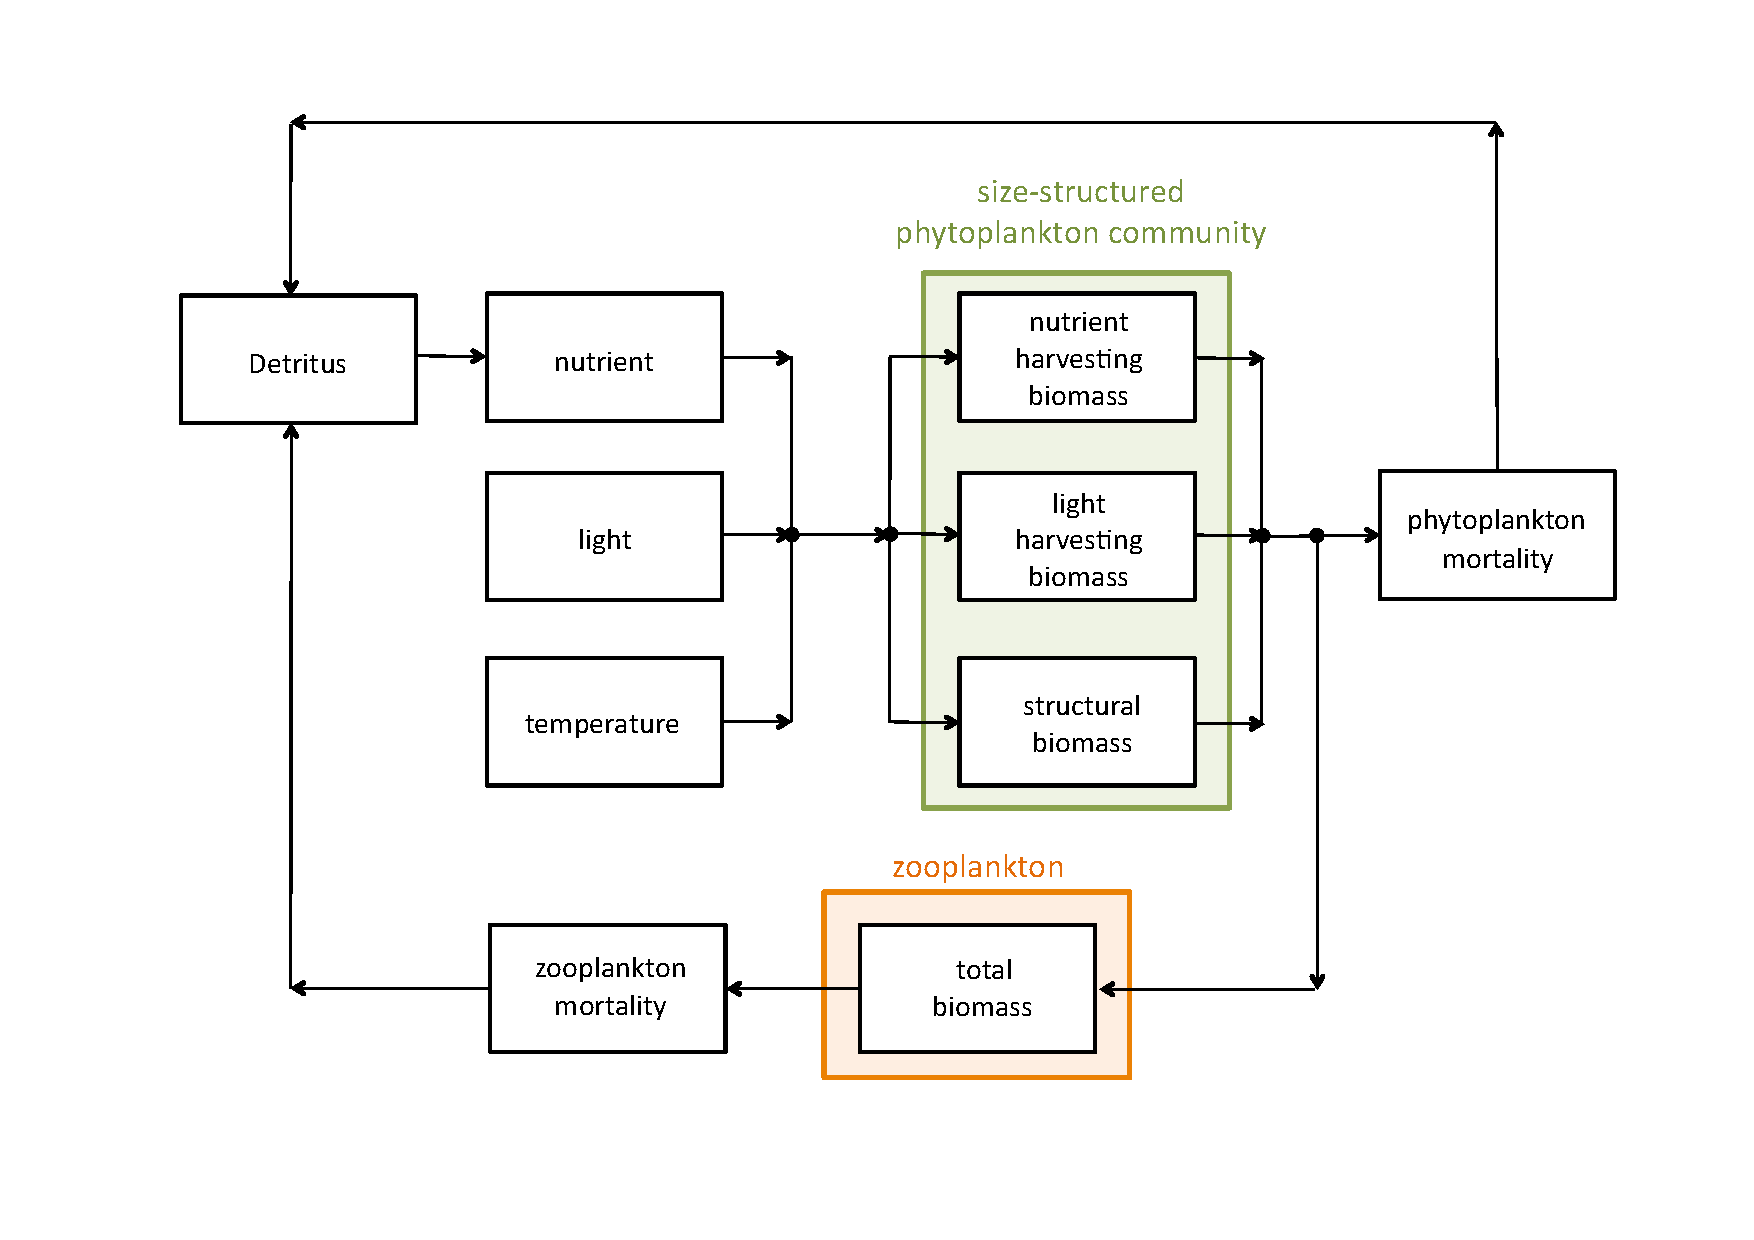
\includegraphics[trim = 15mm 50mm 15mm 25mm, clip, width=1\linewidth]{./Chp3-Further/model-scheme.pdf}
\caption[Scheme]{\small {Scheme of the proposed size-based model. In this model phytoplankton allocates energy (or biomass) to different pools such as nutrient and light harvesting biomasses and generic structural biomass. A certain fraction of the phytoplankton biomass flows into the zooplankton biomass and a remaining fraction is remineralized into the nutrient pool}}
\label{model}
\end{figure}

\begin{figure}
\centering
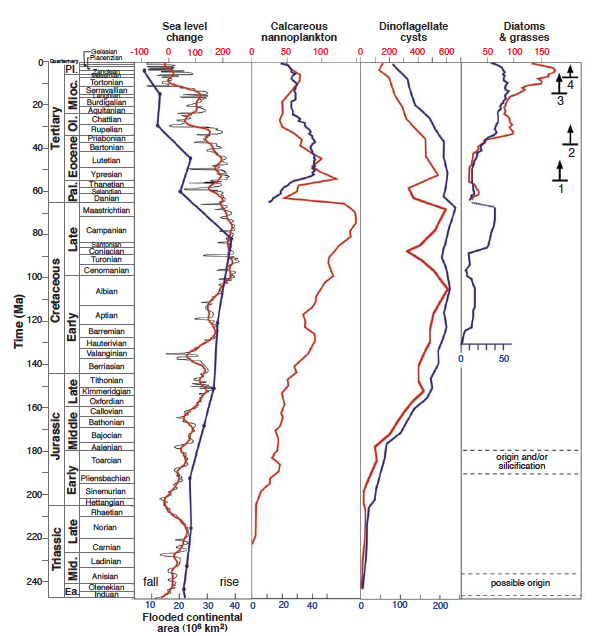
\includegraphics[trim = 0mm 0mm 0mm 0mm, clip, width=1\linewidth]{./Chp3-Further/Falkowski-2004.png}
\caption[Scheme]{\small {Comparison of major phytoplankton groups with sea-level change. The red line accounts for species diversities from published studies. The blue line accounts for the genus diversity compiled from public databases by the authors. Taken from \citet{Falkowski2004a}. }}
\label{Falkowski}
\end{figure}



%%%% TABLES %%%%

\begin{table}
\centering
\caption[Scheme]{\small {Mean values of environmental parameters for the different clusters: High temperature - Low nutrients (HTLN), Mid temperature - Low nutrients (MTLN), Mid temperature - High nutrients (MTHN and Low temperature - High nutrients (LTHN).}}
\label{tableclus}
\begin{tabular} {c c c c c}
cluster & NO$_2^-$ + NO$_3^-$ & PO$_4^{3-}$ & SiO$_4^{2-}$ & Temperature \\ \hline
HTLN & 0.150$\pm$0.575 & 0.064$\pm$0.078 & 1.097$\pm$0.575 & 25.299$\pm$2.000 \\
MTLN & 0.556$\pm$1.102 & 0.112$\pm$0.141 & 0.816$\pm$0.617 & 17.894$\pm$2.191 \\
MTHN & 9.027$\pm$3.593 & 0.799$\pm$0.373 & 2.423$\pm$1.375 & 11.925$\pm$2.797 \\
LTHN & 30.324$\pm$4.549 & 1.336$\pm$0.208 & 4.590$\pm$1.926 & 6.810$\pm$3.435 \\ \hline
\end{tabular}
\end{table}



\begin{table}
\centering
\caption[Scheme]{\small {Summary statistics for linear fittings of the three size fractions to each environmental variable.}}
\label{stats}
\begin{tabular} {c c c c c c c c c c }
& \multicolumn{3} {c} {Picoplankton} & \multicolumn{3} {c} {Nanoplankton} & \multicolumn{3} {c} {Microplankton} \\
& slope & p-value & $r^2$ & slope & p-value & $r^2$ & slope & p-value & $r^2$ \\ \hline
NO$_2^-$ + NO$_3^-$ &-0.090 &0.002 & 0.908 &0.050 &0.001 & 0.921 &0.040 &0.010 &0.792 \\
PO$_4^{3-}$ &-0.0812 &0.021 &0.711 &0.042 &0.012 &0.777 &0.039 &0.125 &0.354 \\
SiO$_4^{2-}$ &-0.047 &0.085 &0.455 &0.030 &0.044 &0.597 &0.016 &0.247 &0.142 \\ 
Temperature &0.082 &0.001 &0.914 &-0.047 &0.008 &0.812 &-0.035 &0.003 &0.885 \\
Copepods &-0.063 &0.064 &0.520 &0.068 &0.051 &0.567 &-0.004 &0.788 &-0.222\\ \hline
\end{tabular}
\end{table}

%%%% typical text %%%%

Smaller phytoplankton cell sizes have a competitive advantage over larger phytoplankton under low nutrient, low light and low grazing pressure \citep{Litchman2008, Litchman2010}. From our regression analyses (Figures \ref{response1} and \ref{response2}) we inferred a strong control of NO$_3^-$+NO$_2^-$ and temperature on all three size fractions. Pico- and nanoplankton size fractions, however, appeared more sensitive to changes in PO$_4^{3-}$, SiO$_4^{2-}$ and copepod abundance. We propose that these effects are caused by a trade-off between resource acquisition and predation pressure, although with the caveat represented by the paucity of the zooplankton data and by the qualitative value we attribute to zooplankton abundance as an indication of grazing pressure. There are a number of important physiological and ecological processes that strongly depend on phytoplankton cell size \citep{Kiorboe1993, Cermeno2008a, Finkel2009a}, including metabolic rates, maximum nutrient uptake rate, nutrient diffusion, light absorption, sinking velocity, trophic interactions and even diversity within taxa, which is often a log-normal distribution of body size. Our results are therefore consistent with this general "size rule" \citep{Finkel2009a}. To our knowledge it is the first time that this feature is observed in data extending across an entire ocean basin and irrespective of temporal changes.


\end{document}
